% Template for PLoS% Version 3.5 March 2018
%
% % % % % % % % % % % % % % % % % % % % % %
%
% -- IMPORTANT NOTE
%
% This template contains comments intended 
% to minimize problems and delays during our production 
% process. Please follow the template instructions
% whenever possible.
%
% % % % % % % % % % % % % % % % % % % % % % % 
%
% Once your paper is accepted for publication, 
% PLEASE REMOVE ALL TRACKED CHANGES in this file 
% and leave only the final text of your manuscript. 
% PLOS recommends the use of latexdiff to track changes during review, as this will help to maintain a clean tex file.
% Visit https://www.ctan.org/pkg/latexdiff?lang=en for info or contact us at latex@plos.org.
%
%
% There are no restrictions on package use within the LaTeX files except that 
% no packages listed in the template may be deleted.
%
% Please do not include colors or graphics in the text.
%
% The manuscript LaTeX source should be contained within a single file (do not use \input, \externaldocument, or similar commands).
%
% % % % % % % % % % % % % % % % % % % % % % %
%
% -- FIGURES AND TABLES
%
% Please include tables/figure captions directly after the paragraph where they are first cited in the text.
%
% DO NOT INCLUDE GRAPHICS IN YOUR MANUSCRIPT
% - Figures should be uploaded separately from your manuscript file. 
% - Figures generated using LaTeX should be extracted and removed from the PDF before submission. 
% - Figures containing multiple panels/subfigures must be combined into one image file before submission.
% For figure citations, please use "Fig" instead of "Figure".
% See http://journals.plos.org/plosone/s/figures for PLOS figure guidelines.
%
% Tables should be cell-based and may not contain:
% - spacing/line breaks within cells to alter layout or alignment
% - do not nest tabular environments (no tabular environments within tabular environments)
% - no graphics or colored text (cell background color/shading OK)
% See http://journals.plos.org/plosone/s/tables for table guidelines.
%
% For tables that exceed the width of the text column, use the adjustwidth environment as illustrated in the example table in text below.
%
% % % % % % % % % % % % % % % % % % % % % % % %
%
% -- EQUATIONS, MATH SYMBOLS, SUBSCRIPTS, AND SUPERSCRIPTS
%
% IMPORTANT
% Below are a few tips to help format your equations and other special characters according to our specifications. For more tips to help reduce the possibility of formatting errors during conversion, please see our LaTeX guidelines at http://journals.plos.org/plosone/s/latex
%
% For inline equations, please be sure to include all portions of an equation in the math environment.  For example, x$^2$ is incorrect; this should be formatted as $x^2$ (or $\mathrm{x}^2$ if the romanized font is desired).
%
% Do not include text that is not math in the math environment. For example, CO2 should be written as CO\textsubscript{2} instead of CO$_2$.
%
% Please add line breaks to long display equations when possible in order to fit size of the column. 
%
% For inline equations, please do not include punctuation (commas, etc) within the math environment unless this is part of the equation.
%
% When adding superscript or subscripts outside of brackets/braces, please group using {}.  For example, change "[U(D,E,\gamma)]^2" to "{[U(D,E,\gamma)]}^2". 
%
% Do not use \cal for caligraphic font.  Instead, use \mathcal{}
%
% % % % % % % % % % % % % % % % % % % % % % % % 
%
% Please contact latex@plos.org with any questions.
%
% % % % % % % % % % % % % % % % % % % % % % % %

\documentclass[10pt,letterpaper]{article}
\usepackage[top=0.85in,left=2.75in,footskip=0.75in]{geometry}

% amsmath and amssymb packages, useful for mathematical formulas and symbols
\usepackage{amsmath,amssymb}

% Use adjustwidth environment to exceed column width (see example table in text)
\usepackage{changepage}

% Use Unicode characters when possible
\usepackage[utf8x]{inputenc}

% textcomp package and marvosym package for additional characters
\usepackage{textcomp,marvosym}

% cite package, to clean up citations in the main text. Do not remove.
\usepackage{cite}

% Use nameref to cite supporting information files (see Supporting Information section for more info)
\usepackage{nameref,hyperref}

% line numbers
\usepackage[right]{lineno}

% ligatures disabled
\usepackage{microtype}
\DisableLigatures[f]{encoding = *, family = * }

% color can be used to apply background shading to table cells only
\usepackage[table]{xcolor}

% array package and thick rules for tables
\usepackage{array}

% text style packages
\usepackage{soul}

%comments (Yarden) margin was changed to accomodate longer text in todos
\usepackage[colorinlistoftodos, textwidth=2in]{todonotes}
%\usepackage[disable]{todonotes}
\reversemarginpar
\setlength{\marginparwidth}{2in}
% create "+" rule type for thick vertical lines
\newcolumntype{+}{!{\vrule width 2pt}}

% create \thickcline for thick horizontal lines of variable length
\newlength\savedwidth
\newcommand\thickcline[1]{%
  \noalign{\global\savedwidth\arrayrulewidth\global\arrayrulewidth 2pt}%
  \cline{#1}%
  \noalign{\vskip\arrayrulewidth}%
  \noalign{\global\arrayrulewidth\savedwidth}%
}

% \thickhline command for thick horizontal lines that span the table
\newcommand\thickhline{\noalign{\global\savedwidth\arrayrulewidth\global\arrayrulewidth 2pt}%
\hline
\noalign{\global\arrayrulewidth\savedwidth}}


% Remove comment for double spacing
%\usepackage{setspace} 
%\doublespacing

% Text layout
\raggedright
\setlength{\parindent}{0.5cm}
\textwidth 5.25in 
\textheight 8.75in
\usepackage{ragged2e}
\usepackage[rightcaption]{sidecap}

% Bold the 'Figure #' in the caption and separate it from the title/caption with a period
% Captions will be left justified
\usepackage[aboveskip=1pt,labelfont=bf,labelsep=period,justification=raggedright,singlelinecheck=off]{caption}
\renewcommand{\figurename}{Fig}

\newcommand{\beginsupplement}{%
        \setcounter{table}{0}
        \renewcommand{\thetable}{S\arabic{table}}%
        \setcounter{figure}{0}
        \renewcommand{\thefigure}{S\arabic{figure}}%
     }

% Use the PLoS provided BiBTeX style
\bibliographystyle{plos2015.bst}

% Remove brackets from numbering in List of References
\makeatletter
\renewcommand{\@biblabel}[1]{\quad#1.}
\makeatother



% Header and Footer with logo
\usepackage{lastpage,fancyhdr,graphicx}
\graphicspath{ {./doc/Figures/} }
\usepackage{epstopdf}
%\pagestyle{myheadings}
\pagestyle{fancy}
\fancyhf{}
%\setlength{\headheight}{27.023pt}
%\lhead{\includegraphics[width=2.0in]{PLOS-submission.eps}}
\rfoot{\thepage/\pageref{LastPage}}
\renewcommand{\headrulewidth}{0pt}
\renewcommand{\footrule}{\hrule height 2pt \vspace{2mm}}
\fancyheadoffset[L]{2.25in}
\fancyfootoffset[L]{2.25in}
\lfoot{\today}

%% Include all macros below
\newcommand{\todoycgr}[1]{
\todo[bordercolor=green, color=green!40, size=\small]{#1}
}

\newcommand{\todoycpu}[1]{
\todo[bordercolor=purple, color=purple!40, size=\small]{#1}
}

\newcommand{\tododnor}[1]{
\todo[bordercolor=orange, color=orange!40, size=\small]{#1}
}

\newcommand{\todotg}[1]{
\todo[bordercolor=yellow, color=yellow!40, size=\small]{#1}
}

%% END MACROS SECTION


\begin{document}
\vspace*{0.2in}

% Title must be 250 characters or less.
\begin{flushleft}
{\Large
\textbf\newline{TweetyNet: A neural network that enables high-throughput, automated annotation of birdsong}
% Please use "sentence case" for title and headings (capitalize only the first word in a title (or heading), the first word in a subtitle (or subheading), and any proper nouns).
}
\newline
% Insert author names, affiliations and corresponding author email (do not include titles, positions, or degrees).
\\
Yarden Cohen\textsuperscript{1\Yinyang*},
David Nicholson\textsuperscript{2\Yinyang},
Alexa Sanchioni\textsuperscript{1},
Emily K. Mallaber\textsuperscript{1},
Viktoriya Skidanova\textsuperscript{1}, 
Timothy J. Gardner\textsuperscript{3\ddag}
\\
\bigskip
\textbf{1} Biology department, Boston University, Boston, MA, USA
\\
\textbf{2} Biology department, Emory University, Atlanta, GA, USA
\\
\textbf{3} Phil and Penny Knight Campus for Accelerating Scientific Impact, University of Oregon, Eugene, OR, USA
\\
\bigskip

% Insert additional author notes using the symbols described below. Insert symbol callouts after author names as necessary.
% 
% Remove or comment out the author notes below if they aren't used.
%
% Primary Equal Contribution Note
\Yinyang These authors contributed equally to this work.

% Additional Equal Contribution Note
% Also use this double-dagger symbol for special authorship notes, such as senior authorship.
% \ddag These authors also contributed equally to this work.

% Current address notes
% \textcurrency Current Address: Dept/Program/Center, Institution Name, City, State, Country % change symbol to "\textcurrency a" if more than one current address note
% \textcurrency b Insert second current address 
% \textcurrency c Insert third current address

% Deceased author note
% \dag Deceased

% Group/Consortium Author Note
% \textpilcrow Membership list can be found in the Acknowledgments section.

% Use the asterisk to denote corresponding authorship and provide email address in note below.
* ycohen1@mgh.harvard.edu
\ddag timg@uoregon.edu
% \todoycgr{Yarden Cohen, GREEN - small comments that are not critical}
% \todoycpu{Yarden Cohen, PURPLE, large comments  comments that are important}
% \tododnor{David Nicholson, ORANGE, comment}
% \todotg{Tim G, YELLOW, comment}
\end{flushleft}
\justify
% Please keep the abstract below 300 words
\section*{Abstract}

Songbirds have long been studied as a model system of sensory-motor learning. Many analyses of birdsong require time-consuming manual annotation of the individual elements of song, known as syllables or notes. Here we describe the first automated algorithm for birdsong annotation that is applicable to complex song such as canary song. We developed a neural network architecture, “TweetyNet”, that is trained with a small amount of hand-labeled data using supervised learning methods. We first show TweetyNet achieves significantly lower error on Bengalese finch song than a similar method, using less training data, and maintains low error rates across days. Applied to canary song, TweetyNet achieves fully automated annotation of canary song, accurately capturing the complex statistical structure previously discovered in a manually annotated dataset.  We conclude that TweetyNet will make it possible to ask a wide range of new questions focused on complex songs where manual annotation was impractical.

% Please keep the Author Summary between 150 and 200 words
% Use first person. PLOS ONE authors please skip this step. 
% Author Summary not valid for PLOS ONE submissions.   
% \section*{Author summary}
% TBD \todoycpu{suggest not including this section for biorxiv - it is journal specific}
\linenumbers

% Use "Eq" instead of "Equation" for equation citations.
\section*{Introduction}
\label{intro}
Songbirds provide an excellent model system for investigating sensorimotor learning \cite{mooney_neurobiology_2009}. 
Like many motor skills, 
birdsong consists of highly stereotyped gestures executed in a sequence \cite{fee_songbird_2010}.
In this and many other ways, birdsong resembles speech: 
 song is learned by juveniles from a tutor, like babies learning to talk \cite{brainard_what_2002}.
A key advantage of songbirds as a model system for studying vocal learning is that birds sing spontaneously, 
often producing hundreds or thousands of song bouts a day.
This provides a detailed readout of how song is acquired during development, 
and how this skilled behavior is maintained in adulthood.
Leveraging the amount of data that songbirds produce requires 
methods for high-throughput automated analyses.
For example, automated methods for measuring similarity of juvenile and tutor song 
across development \cite{tchernichovski_procedure_2000,mets_automated_2018}
led to important advances in understanding the behavioral 
\cite{tchernichovski_dynamics_2001,mets_learning_2019}
and genetic \cite{mets_genetic_2018} bases of how vocalizations are learned.
These examples demonstrate how automated methods that enable analysis of 
large-scale behavioral datasets 
contribute to realizing the potential of songbirds as a model system.

However, this potential to address central questions of sensorimotor learning 
is currently hindered by a lack of high-throughput automated methods  
for scaling up other types of analyses.
The central issue is that many analyses require researchers to annotate song.
Annotation is a time-consuming process done by hand 
(typically with GUI-based applications, e.g., Praat, Audacity, Chipper  \cite{noauthor_praat_nodate,noauthor_audacity_nodate, searfoss2020chipper}).
An example of Bengalese finch song annotated with a GUI is shown in Fig.~\ref{fig0}.
Researchers annotate song by dividing it up into segments (red lines in Fig.~\ref{fig0}), 
often referred to as syllables or notes, 
and assigning labels to those segments (letters in Fig.~\ref{fig0}).
Annotation makes several types of analyses possible. 
For example, annotation is required to build statistical models of syntax
\cite{markowitz_long-range_2013,jin2011compact,berwick2011songs,hedley2016complexity},
to fit computational models of motor learning that 
precisely quantify how single syllables change over the course of an experiment
\cite{sober2009adult,sober2012vocal}, 
and to relate behavior to neural activity 
\cite{wohlgemuth_linked_2010,aronov_specialized_2008,hahnloser_ultra-sparse_2002}.
Annotating song greatly increases our ability to leverage songbirds as a model system 
when answering questions about how the brain produces syntax observed in 
sequenced motor skills, and how the brain learns to adaptively control muscles.

\begin{figure}[!ht]
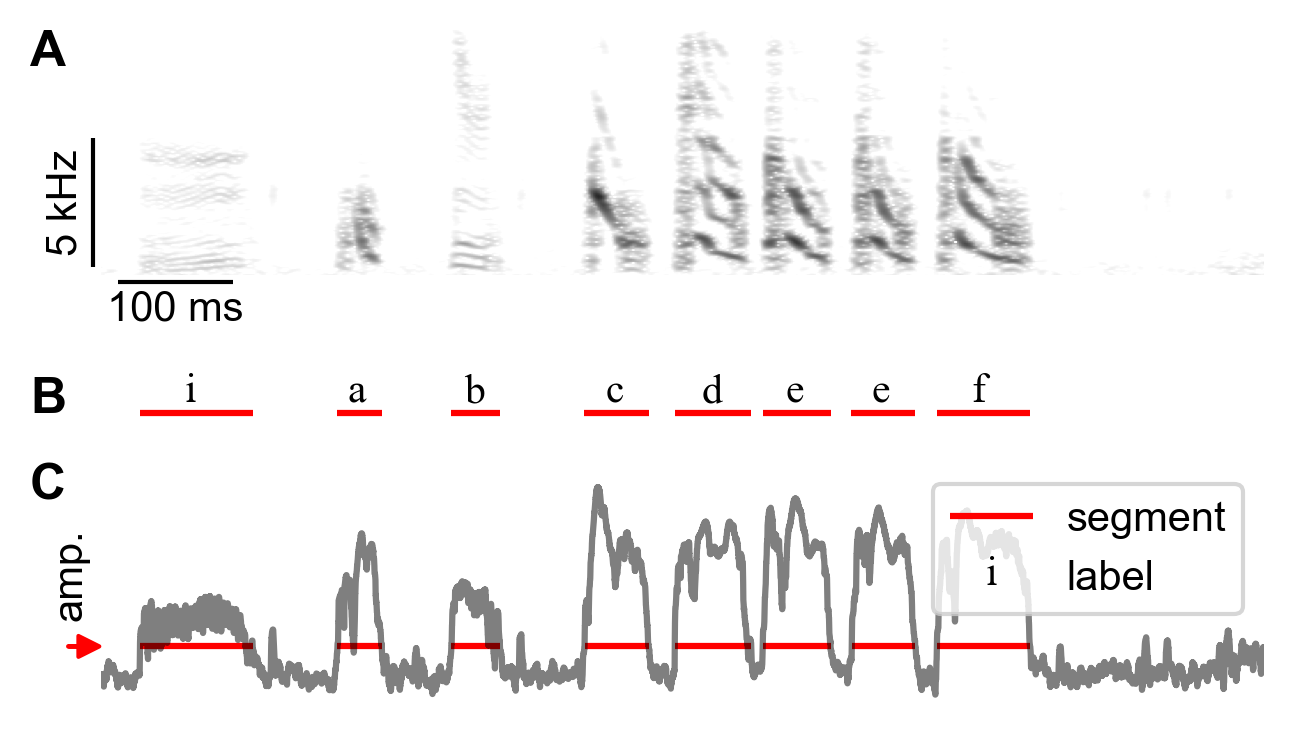
\includegraphics[scale=1.0]{Figures/fig0/annotfig.png}
\caption{{\bf Annotation of birdsong.}
\textbf{A.} Spectrogram showing a brief clip of Bengalese finch song 
with different syllable types. 
\textbf{B.} Text labels over red segments are applied by human annotators to assign those segments to various syllable classes.
\textbf{C.} Segments were extracted from song by finding continuous periods above a fixed amplitude threshold.
Red arrow to left of panel \textbf{C} indicates the user-defined amplitude threshold.
}
\label{fig0}
\end{figure} 

Previous work has been done on automating annotation, 
as we briefly review below in \nameref{Related work},
but these methods are challenged by the variable song of some species.
To illustrate these challenges,  Fig~\ref{fig1}A-C presents examples of annotated songs from different species.
When a species' song consists of just a few syllables sung repeatedly in a fixed motif, methods based on template matching or 
other algorithms (see \nameref{Related work} below) can be applied.
This is true for zebra finches, as can be seen in a song from one individual shown in Fig~\ref{fig1}A.
However, many species have songs that are more complex than the stereotyped motif of zebra finches.
Complex songs can contain a large vocabulary of syllable types arranged in multiple motifs or phrases, 
with phrases sequenced according to complex transition statistics. For example, Bengalese
finch song contains "branch points", where a given syllable may transition to more than one other class of
syllable. An example of a branch point is indicated above the spectrogram in Fig~\ref{fig1}B. In addition,
Bengalese finch song can contain syllables that repeat, with the number of repeats varying from rendition to
rendition. Both branch points and repeats prevent existing algorithms from effectively annotating Bengalese
finch song (Fig~\ref{fig1}E). Canary song is even more complex (Fig~\ref{fig1}C). Some individuals may have as many as 50 unique classes of syllables in their repertoire. Bouts of canary song can last more than a minute instead of a few seconds (Fig~\ref{fig1}D). These long songs contain individual syllable types that  can be very short, under 10ms, or very long, ranging up to 500ms (Fig~\ref{fig1}F). Some syllables are very quiet, and others loud.
Because of this extreme range of amplitude, common methods for segmenting audio of song into syllables can fail.
Segments are typically defined as points where the smoothed sound envelope or other song-related acoustic features \cite{tchernichovski_procedure_2000} stay above some threshold, indicated by the dashed lines in Fig \ref{fig2}. In the case of canary song, if sound energy or other acoustic features are filtered on timescales short enough to accurately segment the shortest syllables, then the longest syllables will be subdivided. This problem is also commonly encountered when analyzing the variable songs of young zebra finches. 
Fig~\ref{fig2} illustrates how canary song is difficult to segment in an automated manner. 
Finally, canary song has a hierarchical structure where syllables occur in trilled repetitions, called phrases, that themselves obey long-range syntax rules \cite{markowitz_long-range_2013,gardner_freedom_2005}. Phrases can differ in duration depending on the type of syllable being repeated and similarly inter-syllable silent gaps vary widely in duration (\nameref{S1_Fig}). Because of all this complexity, there are currently no automated methods for accurate annotation of canary song.

\begin{figure}[!ht]
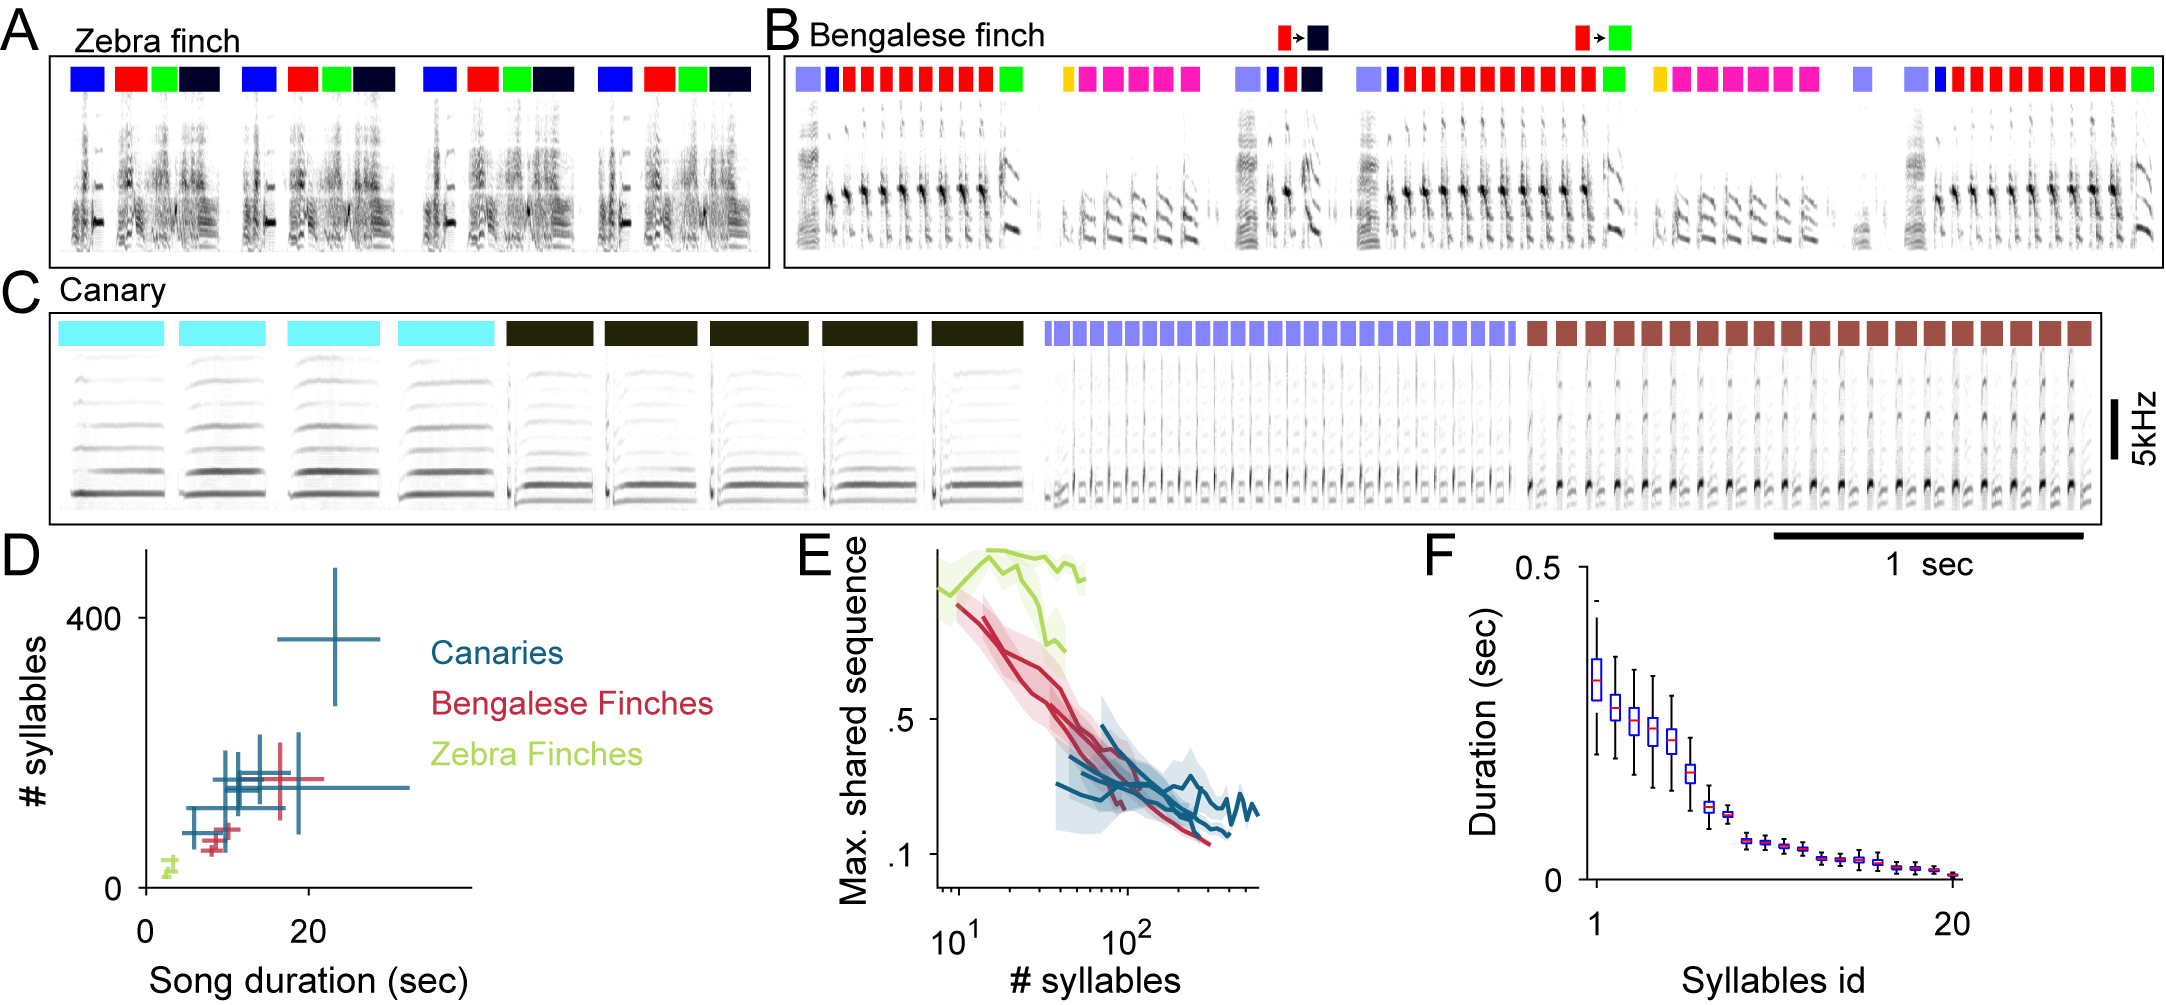
\includegraphics[scale=0.725]{Figures/fig1/Figure1_v4.png}
\caption{{\bf The challenge of annotating complex songs.}
\textbf{A.} The zebra finch repeating motif allows annotation by matching its template spectrogram without segmenting different syllables (colored bars).
\textbf{B.} Bengalese finch songs segmented to syllables shows variable transitions and changing numbers of syllable repeats.
\textbf{C.} A third of one domestic canary song of median duration segmented to syllables reveals repetitions (phrase) structure.  
\textbf{D.} The median, 0.25 and 0.75 quantiles of song durations (x-axis) and # of syllables per song (y-axis) for 2 canary strains, Bengalese finches and Zebra finches (color coded)
\textbf{E.} Variable songs are not suited for template matching. Songs contain repeating sequences of syllables but because of sequence variability songs with more syllables (x-axis) share smaller sequence fractions (y-axis)
\textbf{F.} Distributions of syllable duration for one domestic canary. The bird had 20 different syllable types (x-axis, ordered by mean syllable duration). Box plot shows median, 0.25 and 0.75 quantiles of syllable durations. Whiskers show the entire range.}
\label{fig1}
\end{figure} 

\begin{figure}[!ht]
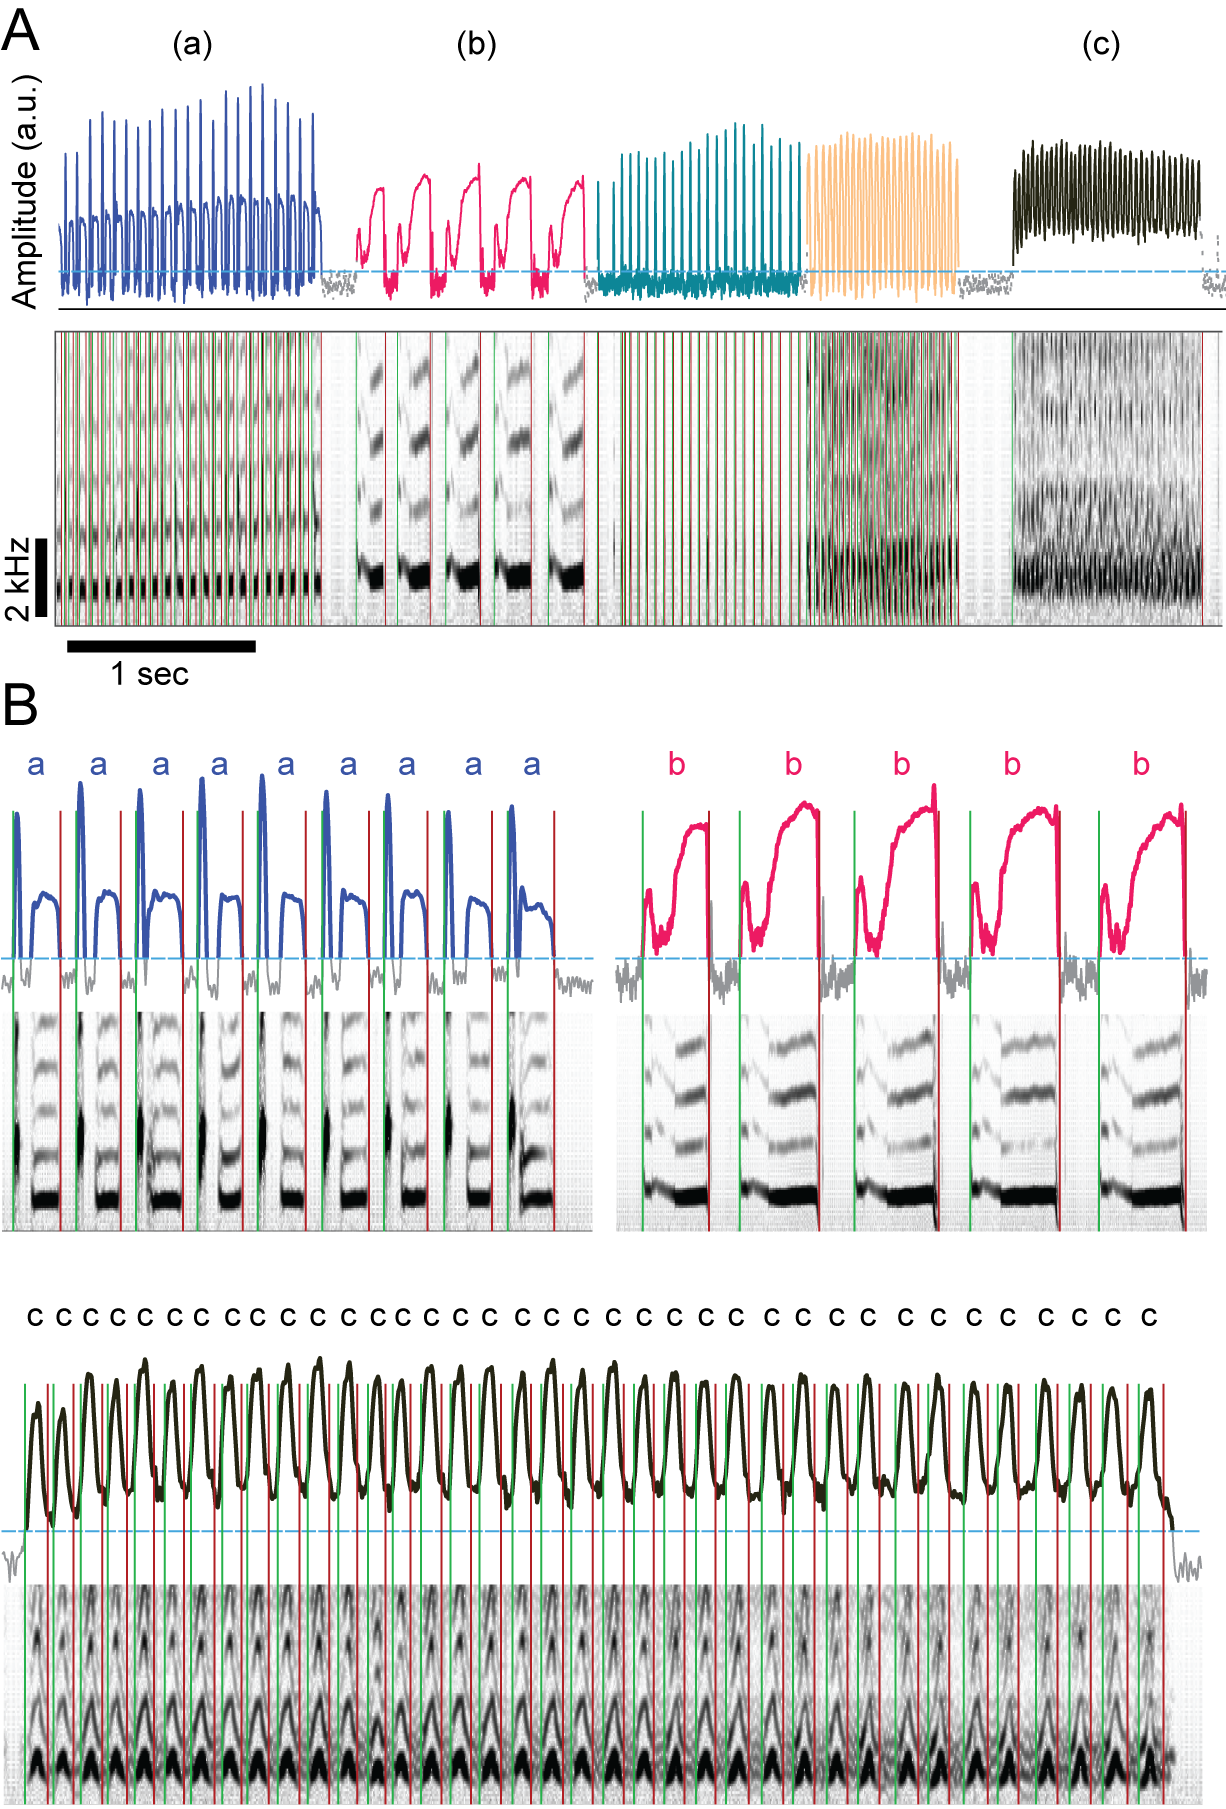
\includegraphics[scale=0.2]{Figures/fig2/fig2_v2.png}
\caption{{\bf Examples of failure to segment canary song.}
\textbf{A.} Several seconds of domestic canary song, presented as a spectrogram, beneath a plot of a band-pass filtered sound amplitude. To segment song, an amplitude threshold can be taken, marked by the dashed line on the amplitude trace, and then an automated program finds continuous segments of above-threshold amplitude and marks the onset and offset times of those segments (green, red lines in the spectrogram panel). 
\textbf{B.} Focusing on three examples (a-c matching panel A), segmenting by threshold crossing with a fixed filtering bandwidth does not work well for canaries.  Above threshold amplitudes are shown in bold colored lines and reveal that syllables of type 'a' are broken into 2 components and syllables of type 'c' are not separated by low amplitude.}
\label{fig2}
\end{figure} 

\subsection*{Proposed Method and Related Work}
\label{Related work}
Previous work has been done to automate annotation, as referenced above, 
that we now briefly review.
The crucial point here is that none of the methods work for canary song, for the 
reasons we outlined and demonstrated in Figs.~\ref{fig1} and~\ref{fig2}, necessitating the 
development of an algorithm like the one we present.
However, for birdsong that consists largely of a single fixed motif, like that of zebra finches,
several methods have been widely used, including semi-automatic clustering methods 
\cite{burkett2015voice,daou2012computational},
and template matching \cite{anderson1996template,yamahachi_undirected_2020,pearre_fast_2017}. 
Several studies have also applied supervised learning algorithms
to annotation, such as Hidden Markov Models \cite{kogan1998automated},
k-Nearest Neighbors \cite{songbrowser}, 
and support vector machines \cite{tachibana2014semi}.
These algorithms can annotate more variable song with branch points and repeats, 
like that of Bengalese finches, 
but they all require segmenting song to extract the engineered features 
used to train the algorithms (e.g. acoustic parameters like pitch and duration).
To our knowledge there has been no large-scale comparison 
of performance of these different algorithms, 
but at least one study suggests they may not generalize well across songs of different 
individuals \cite{nicholson2016comparison}. 
Additionally, feature extraction can fail if segmentation is noisy, 
e.g. because of changes in audio equipment set-up, background noises, etc.
Here again we stress that canary song exhibits wide ranges in amplitude, 
and often requires annotators to set multiple thresholds to successfully extract segments. 
These factors contribute to the lack of automated algorithms for annotating canary song.

Given these issues, we sought to develop an algorithm for automated annotation 
that (1) can learn features from data, and 
(2) does not require segmented syllables to predict annotations.
To meet both these criteria, we developed an artificial neural network 
that we call TweetyNet, shown in (Fig~\ref{fig3}).
TweetyNet takes as input windows from spectrograms of song 
and produces labels for each time bin of that spectrogram window.
TweetyNet requires no pre-processing of song spectrograms - most importantly,  segmentation of song into syllables is not needed. Silent gaps between syllables are labelled in training data, and these silent labels are assigned to gaps between syllables when TweetyNet inference is applied to a new song. 

Essentially, the network combines two types of layers found in neural networks:(1) convolutional layers, common in computer vision tasks to learn features of images \cite{goodfellow_deep_2016,farabet_learning_2013,krizhevsky_imagenet_2012}, and (2) recurrent layers, often used to predict sequences \cite{graves_supervised_2012}. A recurrent layer is a natural choice because the input image or spectrogram is defined by two axes (time and frequency) with very different correlation structure.  Specifically, the temporal dimension of songbird vocalization, like music and environmental noises, contains regularities in multiple time scales that are unrelated to the regularities of the frequency axes. The bidirectional LSTM (Long-Short-Time-Memory) recurrent layer is designed to capture these temporal correlations. \cite{bock_polyphonic_2012-1,parascandolo_recurrent_2016}. 

To predict annotation, we feed consecutive windows from spectrograms to trained networks and
then concatenate the output vectors of labeled timebins. 
Finally, we simply find uninterrupted runs of a single syllable label to annotate song syllables from this framewise classification. As discussed below, this final step can include a "debounce" step that requires a minimum syllable duration and choosing a single label for consecutive time bins not labeled as silence by majority vote. In the rest of the results below we show that this simple method trained end-to-end 
provides robust predictions of segment onsets, offsets, and labels.


\begin{figure}[!ht]
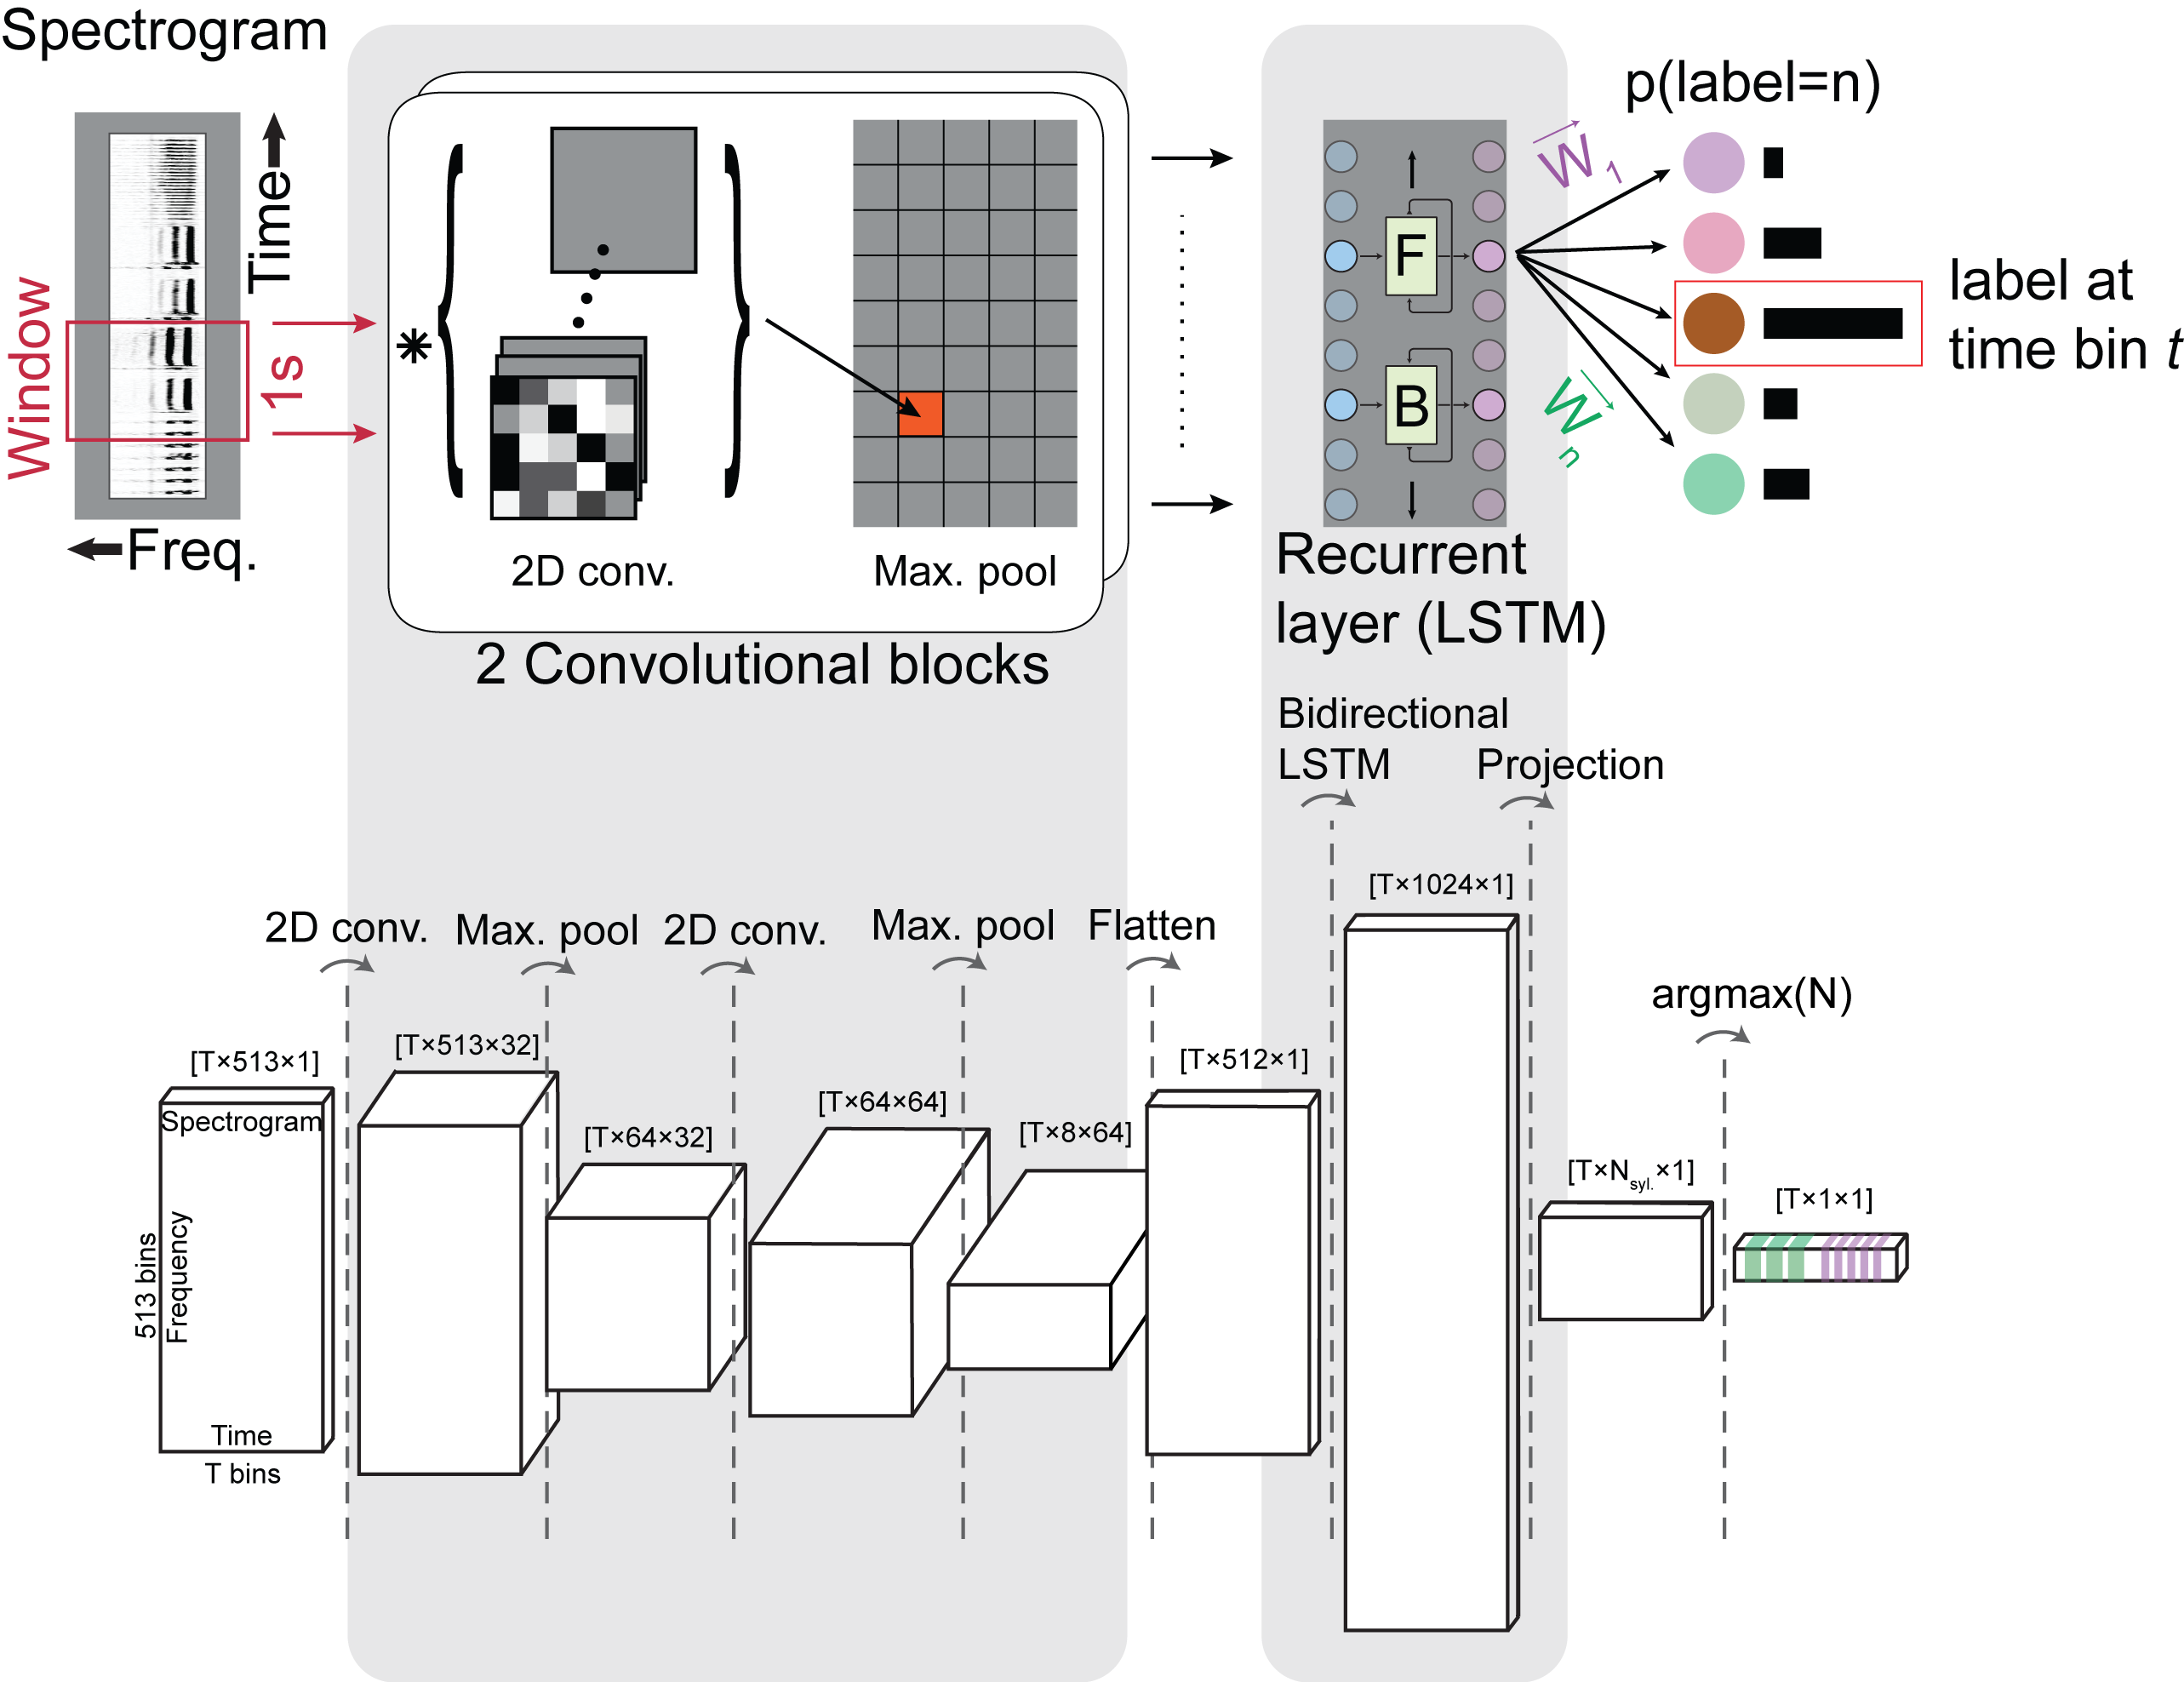
\includegraphics[scale=0.5]{Figures/fig3/fig3_v2.png}
\caption{{\bf TweetyNet neural network architecture.}
Top, network schematic. TweetyNet takes as input a window, 
specified in time bins, from a spectrogram (red box, left) 
and in a sequence of steps (left to right) outputs a label for each time bin within the window:
(1) The convolutional blocks produce a set of feature maps 
by performing a cross-correlation-like operation (asterisk) 
between their input and a set of learned filters (greyscale boxes). 
A max-pooling operation down samples the feature maps.
(2) The recurrent layer is made up of Long Short Term Memory (LSTM) units, 
and the number of units equals the number of time bins in the spectrogram window. 
This step is designed to capture dependencies across time 
using both forward (F) and backward (B) passes through time to learn. 
(3) A projection ($\overrightarrow{W}_{t,s}$) onto the different syllable classes, $s=1..n$, 
resulting in a vector of probabilities at each time bin $t$ that the label is $n$. 
The number of classes, $n$, is predetermined by the user and includes a class for no-song time bins.
(4) Each time bins is labeled by choosing the class with the highest probability 
and the labelled time bins are used to separate continuous song segments 
from no-song segments and to annotate each song-segment with a single label.
Bottom, the shapes of tensors (multi-dimensional arrays) that result from each operation the network performs.}
\label{fig3}
\end{figure}

Surprisingly, beyond the work previously cited, we find little research that addresses the problem of learning to classify each time bin of a vocalization, either for human speech or birdsong.
The architecture we present here is somewhat similar to early deep networks models for speech recognition, 
but a crucial difference is that state-of-the-art models in that area 
map directly from sequences of acoustic features to sequences of words \cite{graves2006connectionist}.
The success of these state-of-the-art models is attributed to the fact that they learn this mapping from speech to text, **avoiding** the intermediate step of classifying each frame of audio, as has previously been shown \cite{graves_supervised_2012}.
In other words, they avoid the problem of classifying every frame that we set out to solve.
The architecture that we develop is most directly related to those that have been used for event 
detection in audio and video \cite{bock_polyphonic_2012-1,parascandolo_recurrent_2016} 
and for phoneme classification and sequence labeling\cite{graves_framewise_2005,graves_supervised_2012}.
The closest prior model for segmenting and labeling birdsong is \cite{koumura_automatic_2016-1}. 
Several aspects of that study provide context for the contributions of our work. 
The authors compared different pipelines that combine a neural network for recognizing syllable 
segments with Hidden Markov Models that learns to predict syllable sequences, and in this way 
improve the output of the network. They measured performance of these pipelines on a large dataset of 
hand-annotated Bengalese finch song which they made publicly available \cite{koumura_birdsongrecognition_2016}.

In summary, the key prior art is the important work of Koumura and Okanoya\cite{koumura_automatic_2016-1}. This work anticipates the overall structure of our model, but through the integration of multiple distinct components that are individually optimized.  In contrast, TweetyNet is a single neural network trained end-to-end, meaning it does not require optimizing multiple models. 
Below we show that TweetyNet meets our criteria for an algorithm that 
learns features from data and does not require segmented song to make predictions.
To do so we we benchmark TweetyNet on Bengalese finch and canary song, 
and where possible compare the performance to \cite{koumura_automatic_2016-1}. 
Additionally we show that we achieve robust performance:
across songs of individuals, which can vary widely even within a species; 
across many bouts of song from one individual, e.g. across days of song, and; 
across multiple species.
Lastly we show that this performance required only a small amount of 
manually annotated data to train TweetyNet models accurately enough to recreate and add details to the deep structure of canary syntax.

\section*{Results}
\label{Results}

\subsection*{TweetyNet annotates Bengalese finch song with low error rates across individuals.}
We first set out to test whether our network robustly annotates syllables across a large number of
individual birds. To do so, we made use of the  
publicly available repository of Bengalese Finch song \cite{koumura_birdsongrecognition_2016},
used to benchmark hybrid neural network-HMM models from \cite{koumura_automatic_2016-1} 
as referenced in \nameref{Related work}. 
The repository contains song from 10 individual birds, with hundreds of bouts of hand-annotated 
song for each bird. Each individual's song had different number of syllables and obeyed a different syntax.
To benchmark TweetyNet models on this dataset, we generated learning curves that plot error of the 
model as a function of the size of the training set (duration in seconds). 
The learning curves give us an estimate of the smallest amount of hand-labeled training data 
we would need to obtain the lowest error that the TweetyNet model can achieve.
For each bird we split the data into fixed training and test sets, 
with durations of 900 and 400 seconds respectively.
Then for each training set duration we trained 10
replicates with a randomly-drawn subset of the training data. 
We computed error metrics for each training replicate on the 
held-out test set for each individual. (See \nameref{Methods} for details.)
As shown in Fig~\ref{fig4}, these learning curves 
demonstrate that TweetyNet models achieved low error rates across all ten birds.
We first looked at frame error, a percentage that measures the number of times the label 
predicted by the model for each time bin in a spectrogram 
did not match the ground truth label.
For all birds %Fig~\ref{fig4}\textbf{A} that for all birds (solid colored lines) 
TweetyNet models achieve less than 8\% frame error with the smallest training set duration 
of 30 seconds (Fig~\ref{fig4}A). 
From the learning curve we can estimate that across birds, the lowest frame error 
that TweetyNet models produce is roughly 4\%, and that they achieve this with just 
180 seconds (three minutes) of training data. (For specific values, see Table~\ref{table:1}.)
Larger training sets did not further reduce error.

% \todotg{The next paragraph doesn't make sense unless you have convereted frame labels to syllable sequences. That hasn't been explained yet. THis could a be a good place to insert a figure with the output vectors alighed to bengalese finch song, and a third panel showing the syllable segmentation and annotation marks.}
To better understand how well the network segments and labels songs, we used another metric, the syllable error rate, which is analogous to the word error rate that is widely used in the speech recognition literature. This metric is an edit distance that counts the number of edits (insertions and deletions) needed to convert a predicted sequence of syllables into the ground-truth sequence. The error rate is normalized by dividing it by the length of the sequences for comparison across birds (e.g. if one bird sang more syllables per bout than another).
Measuring the syllable error rate confirmed that TweetyNet consistently achieved similar error rates across the ten birds, as shown in 
Fig \ref{fig4}B. Because this metric was also used in \cite{koumura_automatic_2016-1} 
(as "note error rate"), we can compare our results directly to theirs. 
As indicated by blue circles in Fig \ref{fig4}B, the best-performing models in that study achieved syllable
error rates of 0.83 and 0.46 with two and eight minutes of training data, respectively. TweetyNet always
achieved much lower syllable error rates. Taken together, the results from benchmarking TweetyNet on this
dataset indicate that the architecture performs well across the song of many individual birds. In addition, it dramatically outperforms existing models with less training data, and does so while being trained end-to-end
without requiring optimizations of multiple steps in a pipeline.

\begin{figure}[!ht]
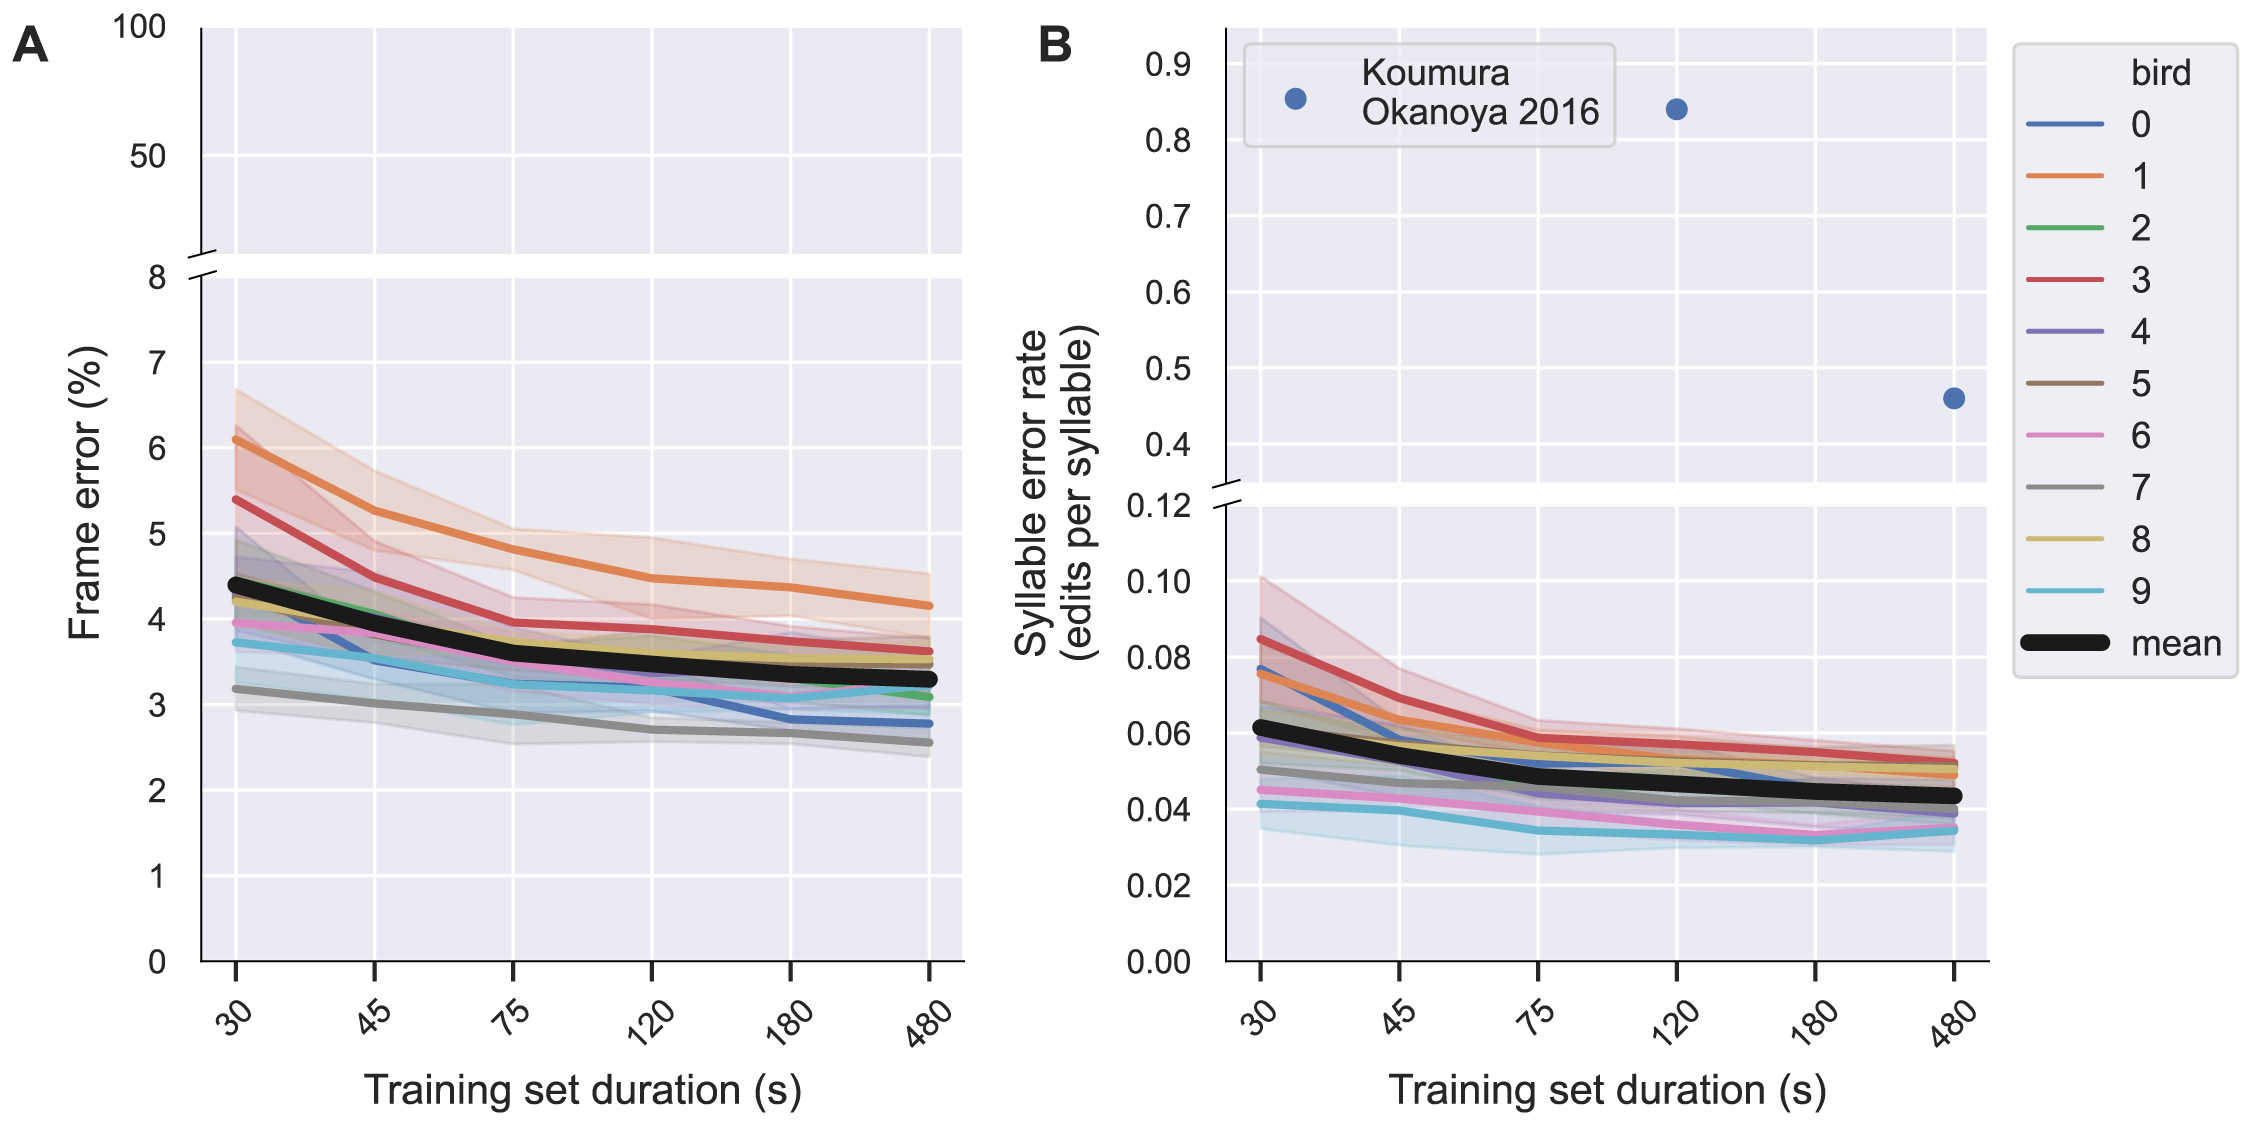
\includegraphics[scale=0.75]{Figures/fig4/fig4-learning-curves-ai.png}
\caption{{\bf TweetyNet annotates song with low error rates across ten indiviudal Bengalese finches.}
Model ‘learning curves’ showing the reduction in annotation error (y-axis) 
on a held-out test set as a function of the size of the training set (x-axis). 
Shown are the ‘frame error rate’ (\textbf{A}) measuring the percent of mislabeled time bins 
and the ‘syllable error rate’ (\textbf{B}) measuring the normalized sequence edit distance. 
Each colored line corresponds to one bird from dataset. 
The solid line indicates mean error across ten training replicates 
for each training set duration, and the translucent error band 
around the solid lines indicates standard deviation. 
Thicker black lines indicate the mean across birds. 
Circular blue markers indicate mean syllable error rate across birds 
reported in \cite{koumura_automatic_2016-1} 
for a different algorithm using the same dataset.}
\label{fig4}
\end{figure}

\subsection*{ TweetyNet models achieve low error across days even when trained with just the first three minutes of song recorded.}
We next sought to benchmark TweetyNet in a scenario similar to long-term behavioral experiments 
for which we hope to automate annotation. 
For this purpose we used another publicly-available repository \cite{nicholson_bengalese_2017} 
with hand-labeled song from four Bengalese finches. 
Importantly, the repository contains most or all of the songs sung 
by each bird for multiple consecutive days, as is typically done 
during a long-term behavioral experiment, 
and annotation for all those songs (recall that experimenters usually are able to annotate only a limited number).
Here we sought to measure how well TweetyNet models 
would perform when an experimenter takes the \textit{first} set of songs of 
some duration $n$ and annotates those songs manually before using them to train a network.
This stands in contrast to the experiment in Fig.~\ref{fig4},
where we trained multiple replicates with random subsets 
of songs from a larger training set, in order to obtain a better estimate of expected error rates.  
Of course our goal is to avoid the need for experimenters to label a large dataset by 
hand and then use it to train multiple replicates with random subsets of that data, 
just to find the best performing network. 
If we show that we can achieve comparable error rates with just the first $n$ minutes of song, we 
can be more confident that TweetyNet models will robustly segment and label hours of song recorded across days.

Using the learning curves in Fig~\ref{fig4} we estimated that three minutes 
of data was the shortest duration training set we could use to obtain 
the lowest error rate achieved by models. 
Thus, we trained single TweetyNet models with the first three minutes of song  
sung by a bird on one day, and then measured the accuracy of 
that model using all other songs across multiple days.
The test datasets we used to obtain these measures were in almost all cases at least as large as 
those we used to benchmark models in the learning curves.
The mean duration of these test datasets was 1528 seconds 
(standard deviation of 888.6 seconds, 
i.e. 25 minutes mean, 14 minutes standard deviation),
in contrast to Fig~\ref{fig4} where we measured error with 
a test set of 400 seconds (6 minutes 40 seconds).
Hence this approach gave us multiple estimates of 
how a single trained model performs on relatively large datasets.
TweetyNet models trained in this manner did achieve low frame error (Fig~\ref{fig5}A) and 
low syllable error rates (Fig~\ref{fig5}B) across days without exhibiting large fluctuations.
The frame error ranged from 2-4\% across 3-5 days of song, 
comparable to those observed when training with a random subset of songs, as in Fig~\ref{fig4}.
In one case, for one bird, the frame error did increase on the last day, but was still 
within the low end of the range seen for all birds, and this increase did not appear to translate into 
an increase in the syllable error rate (Fig~\ref{fig5}B and Fig~\ref{fig5}C, bird ID or60yw70, red line).

We also found that TweetyNet models trained on the first three minutes of song 
maintained a low syllable error rate across days (Fig~\ref{fig5}B and Fig~\ref{fig5}C), 
again comparable to what we observed in the learning curves (Fig~\ref{fig4}B).
Here we additionally tested whether a simple post-processing step could 
further lower the error rate. This "majority vote" transform consists of 
taking each labeled segment (bordered by two segments that the network 
predicted were "unlabeled" / "silent" segments), finding the label 
occurred most frequently within that segment, and then assigning that 
label to all time bins within the segment.
As shown in Fig~\ref{fig5}C, this simple post-processing step 
did lower the syllable error rate of TweetyNet models.
We did not find that this post-processing step had a large effect on the 
frame error (not shown in plot), from which we infer that this 
transform removes small frame errors (e.g. a single time bin) that give 
rise to spurious extra segments, 
and correcting these in turn produces a large drop in the syllable error rate.
Hence we have shown using Bengalese finch song 
that TweetyNet outperforms existing models and that, 
with only minimal cleaning of its output, analyses of behavioral experiments 
can be scaled up to very large datasets.

\begin{figure}[!ht]
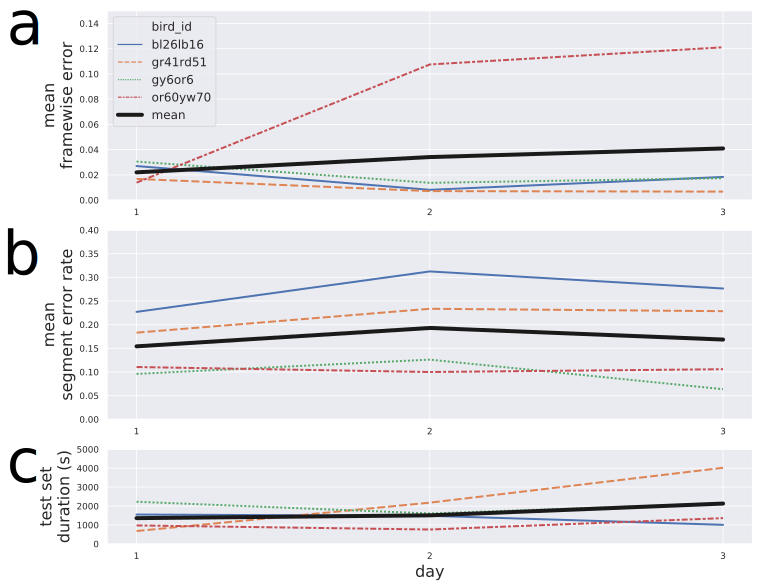
\includegraphics[scale=0.75]{Figures/fig5/fig5-error-across-days-ai.png}
\caption{{\bf TweetyNet models achieve low error across days of Bengalese finch song, 
even when trained with just the first three minutes of song recorded}.
\textbf{A.} TweetyNet models trained on the first three minutes of song 
from day 1 achieved low frame error across days.
The mean duration of the set of songs for each day 
that we used to measure error was 1528 seconds(888.6 S.D.), 
(i.e. 25 minutes (14 minutes S.D.)),
Different line colors and styles indicate individual birds
\textbf{B.} TweetyNet models trained on the first three minutes of song 
from day 1 also demonstrate a low syllable error rate across days.
\textbf{C.}  The syllable error rates in \textbf{B} further improve 
after applying a “majority vote” post-processing 
(assigning the dominant label in each continuous segment of time bins 
not annotated as ‘silence’, see methods).
For one bird (or60yw70), the error did increase on the last day, 
but was still within the low end of the range seen for all birds.
}
\label{fig5}
\end{figure}

\subsection*{TweetyNet annotates minutes-long canary songs with low error rates across individuals}

After demonstrating TweetyNet's high performance across multiple individuals of the same species and across multiple songs of individual birds, we wanted to test TweetyNet across species. We chose the domestic canary (serinus canaria) - a species for which there are no published annotation algorithms and whose rich song repertoire offers a unique opportunity for neuroscience research \cite{markowitz_long-range_2013,gardner_freedom_2005,alonso_low-dimensional_2009,appeltants_effect_2005,alliende_species-specific_2013}.    
 
As in our first test in Bengalese finches, we curated training sets of 1-10 minutes of song from 3 canaries and measured the frame error rates in a held-out test set 20-30 minutes long. (Training sets are relatively longer than the Bengalese tests since canary songs can be up to a minute or more in length and even sparse sampling of the full repertoire requires these longer training sets.)  Still, Fig~\ref{fig6} shows that in three canaries the model learning curves asymptote with 8-10 minute training sets to frame error rates similar to TweetyNet's performance in Bengalese finches.    

\begin{figure}[!ht]
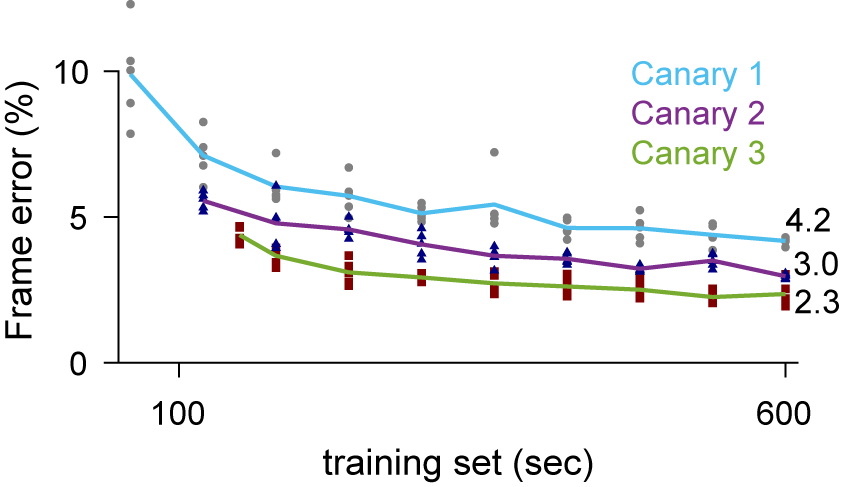
\includegraphics[scale=1.0]{Figures/fig6/fig6_CanaryLC.png}
\caption{{\bf TweetyNet segments and labels canary song with low error rates, similar to Bengalese finches, across individuals.}
Models were trained on 60s-600s of song from each individual. The mean frame error (lines) of five models (markers) trained with different randomly-drawn subsets from the training set was measured on a separate 1500-2000s test set from each individual. The asymptotic error rates, annotated to the right of the curves, overlaps with the error rates in the Bengalese finch data sets}
\label{fig6}
\end{figure}

Unlike TweetyNet's performance in Bengalese finches, the frame error rates in annotating canary songs cannot be compared to alternative algorithms using published data and results. Furthermore, the length of these songs, usually containing hundreds of syllables, mean that even in very low error rates we expect annotation errors in many songs (Table~\ref{table:1}, \nameref{S2_Fig}). These annotation errors can occur at the onset of song and in transitions between canary phrases (Fig~\ref{fig7}) and affect analyses of canary syntax. 

To gauge the effect of such errors, in the next section we evaluate the accuracy of syntax models estimated from TweetyNet's automatic annotation. 
\begin{table}[h!]
\centering
\begin{tabular}{ | c || m{5em} | m{5em} | m{5em} | m{5em} | m{5em} || m{5em} |  }
 \hline
 dataset & training set duration (s) & frame error (\%) & syllable error rate & syllable error rate (majority vote) & \% Near Boundary \\
 \hline
B.F. 1            & 120 & 3.5$\pm$0.5 & 0.05$\pm$0.01 & n/a & n/a\\
\hline
B.F. 1            & 180 & 3.4$\pm$0.5 & 0.04$\pm$0.01 & n/a & n/a\\
\hline
B.F. 1            & 480 & 3.3$\pm$0.5 & 0.04$\pm$0.01 & n/a & n/a\\
\hline
B.F. 2 & 180 & 2.9$\pm$1.4 & 0.2$\pm$0.09 & 0.06$\pm$0.04 & 64.9$\pm$14.3\\
\hline
Can. & 240 & 3.9$\pm$1.0 & 0.155$\pm$0.072 & 0.076$\pm$0.037 & 51.1$\pm$10.7\\
\hline
Can. & 600 & 3.1$\pm$0.8 & 0.09$\pm$0.016 & 0.051$\pm$0.011 & 58.3$\pm$11.3\\
\hline
Can. & 6000 & 2.1$\pm$0.8 & 0.069$\pm$0.013 & 0.031$\pm$0.005 & 68.6$\pm$13.9\\
% Frames  &0&0&0&0&0&0.03&0.012&0.023\\
% \% In-Edge &0&0&0&0&0&84&61&59\\
% Segments  &0&0&0&0&0&0.069&0.056&0.082\\
% Cleaned seg.  &0&0&0&0&0&0.031&0.025&0.037\\
 \hline
\end{tabular}
\caption{{\bf Error metrics of TweetyNet models for different species and training set sizes}
For each Bengalese finch (BF) and canary (Can) data set we evaluate test-set errors metrics for models trained on several training-sets sizes (measured in seconds). Presented are the mean $\pm$ standard deviation across all birds and experiment replicates. The \textit{frame error rate}  and \textit{syllable error rate} columns present the raw error shown in learning curves (Figs.~\ref{fig4},\ref{fig6}). The \textit{syllable error rate (majority vote)} column shows the syllable error rate after applying post-hoc cleaning of annotation, where we assigned a single label to each segment by majority vote and discarded all segments below a set duration (methods). The \textit{\% Near Boundary} column shows the percent of frame errors involving silent periods that occur within 0-2 time bins of syllable boundaries (onsets and offsets, see \nameref{Methods}).}
\label{table:1}
\end{table}


\begin{figure}[!ht]
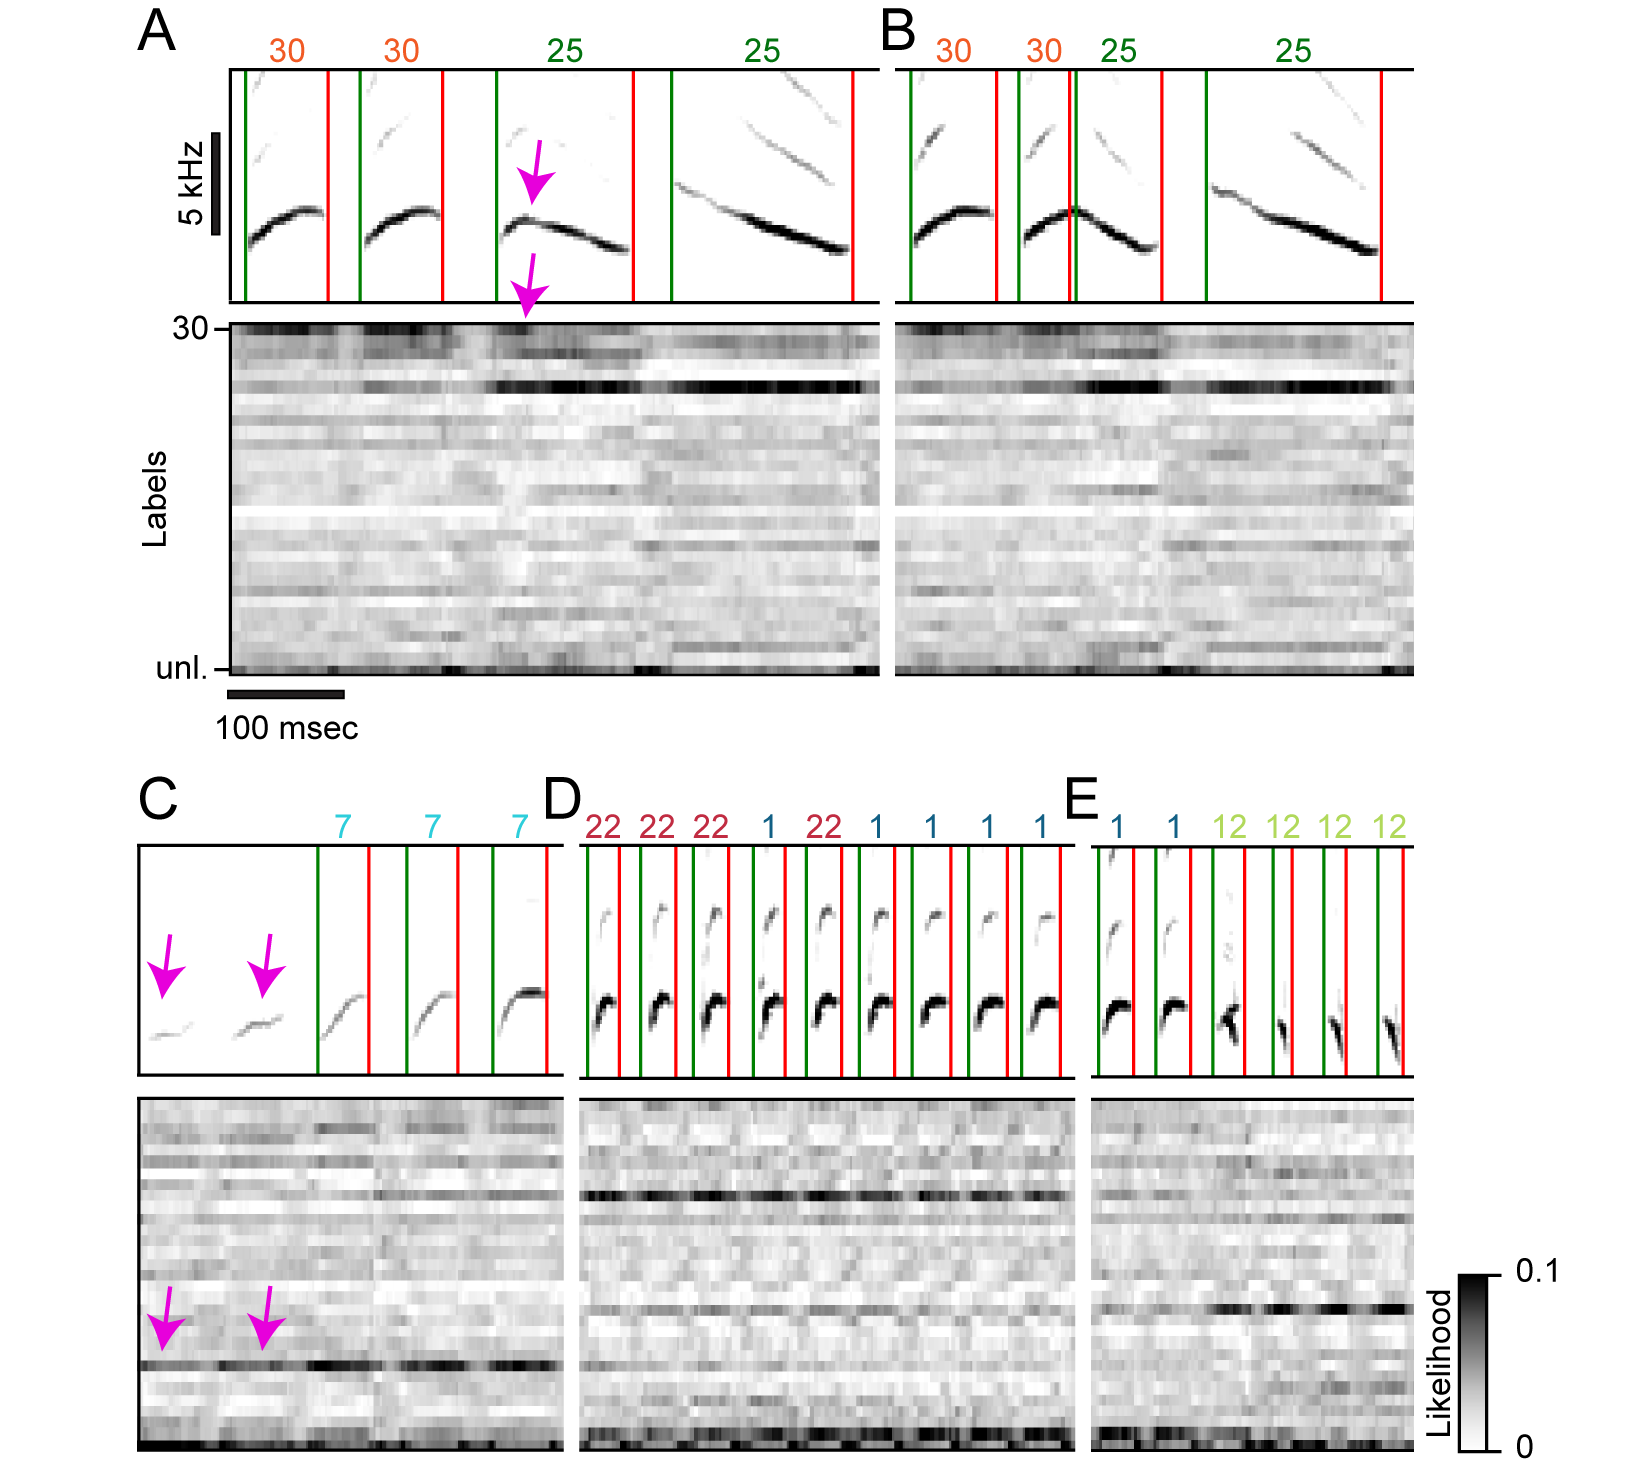
\includegraphics[scale=1.0]{Figures/fig7/fig7_model_err_examples.png}
\caption{{\bf Variants of canary song introduce segmentation and annotation errors.}
Canary vocalizations contain variations that challenge TweetyNet. The examples in panels A-E show spectrograms on top of the time-aligned likelihood (gray scale) assigned by a trained TweetyNet model to each of the labels (y-axis, 30 syllable types and the tag \textit{unl.} for the unlabeled segments). Green and red vertical lines and numbers on top of the spectrograms mark the onset, offset, and labels predicted by the model. 
\textbf{A,B.} Transitions between syllables can occur without a silence gap. In this example, TweetyNet assigns higher likelihood to both syllables (c.f. pink arrow). In rare variants the model ignores the first syllable (A)      
\textbf{C.} Syllables produced weakly or deformed still get higher likelihood (arrows) but may still be ignored because the unlabeled class gets a higher likelihood.
\textbf{D.} Transition between phrases of very similar syllables (22 \textrightarrow 1) introduce label confusion.
\textbf{E.} Canaries can produce completely overlapping syllables. The model assigns high likelihood to both classes but is forced to choose only one}
\label{fig7}
\end{figure}



\subsection*{Automated analysis of canary song structure. }

Sequences of canary phrases contain transitions with different 'memory' depths. Namely, the probability distribution of transition outcomes from a given phrase is captured by Markov chains with variable lengths. As shown in a recent study in Waterslager canaries, this syntax structure is captured parsimoniously by probabilistic suffix trees (PST) \cite{ron_power_1996,markowitz_long-range_2013}. 
The root node in these graphical models, appearing in the middle of Fig~\ref{fig8}A,B and Fig~\ref{fig9}A,B, represents the zero-order Markov, or base rate, frequencies of the different phrases, labelled in different colors and letters. Each branch, emanating from the colored letters in Figs~\ref{fig8},\ref{fig9} represents the set of Markov chains that end in the specific phrase type designated by that label. For example, the 'A' branch in Fig~\ref{fig8}a includes the first order Markov model 'A' and the second order Markov chains 'FA' and '1A' representing the second order dependence of the transition from phrase 'A'.
These models are built by iterative addition of nodes up the branch to represent longer Markov chains, or a transition's dependence on longer sequences of song history. 

Figures~\ref{fig8} and \ref{fig9} demonstrate that TweetyNet parses domestic canary song with an accuracy sufficient to extract its long-range order. In both of these figures, we set parameters of the PST estimation algorithm to derive the deepest syntax structure possible without overfitting as practiced in a recent study \cite{markowitz_long-range_2013} that used about 600 hand annotated songs of Waterslager canaries. In this example, using 2.2\% of the data set, about 40 songs, to train a TweetyNet model and predict the rest of the data reveals the deep structures shown in Fig~\ref{fig8}B - comparable to using 600 hand annotated songs of the same bird (Fig~\ref{fig8}A). With more training data, Tweetynet's accuracy improves as does the statistical strength of the syntax model. In Fig~\ref{fig9}B a TweetyNet model was trained on 19\% of the data, about 340 songs, and predicted the rest of the data. The resulting syntax model can be elaborated to greater depth without overfitting. To crosscheck this deeper model, we manually annotated all 1764 songs of that bird, revealing a very similar syntax model (Fig~\ref{fig9}A).


In sum, we find that TweetyNet, trained on a small sample of canary song, is accurate enough to automatically derive the deep structure that has formed the basis of recent studies \cite{markowitz_long-range_2013,cohen_hidden_2020}.




\begin{figure}[!ht]
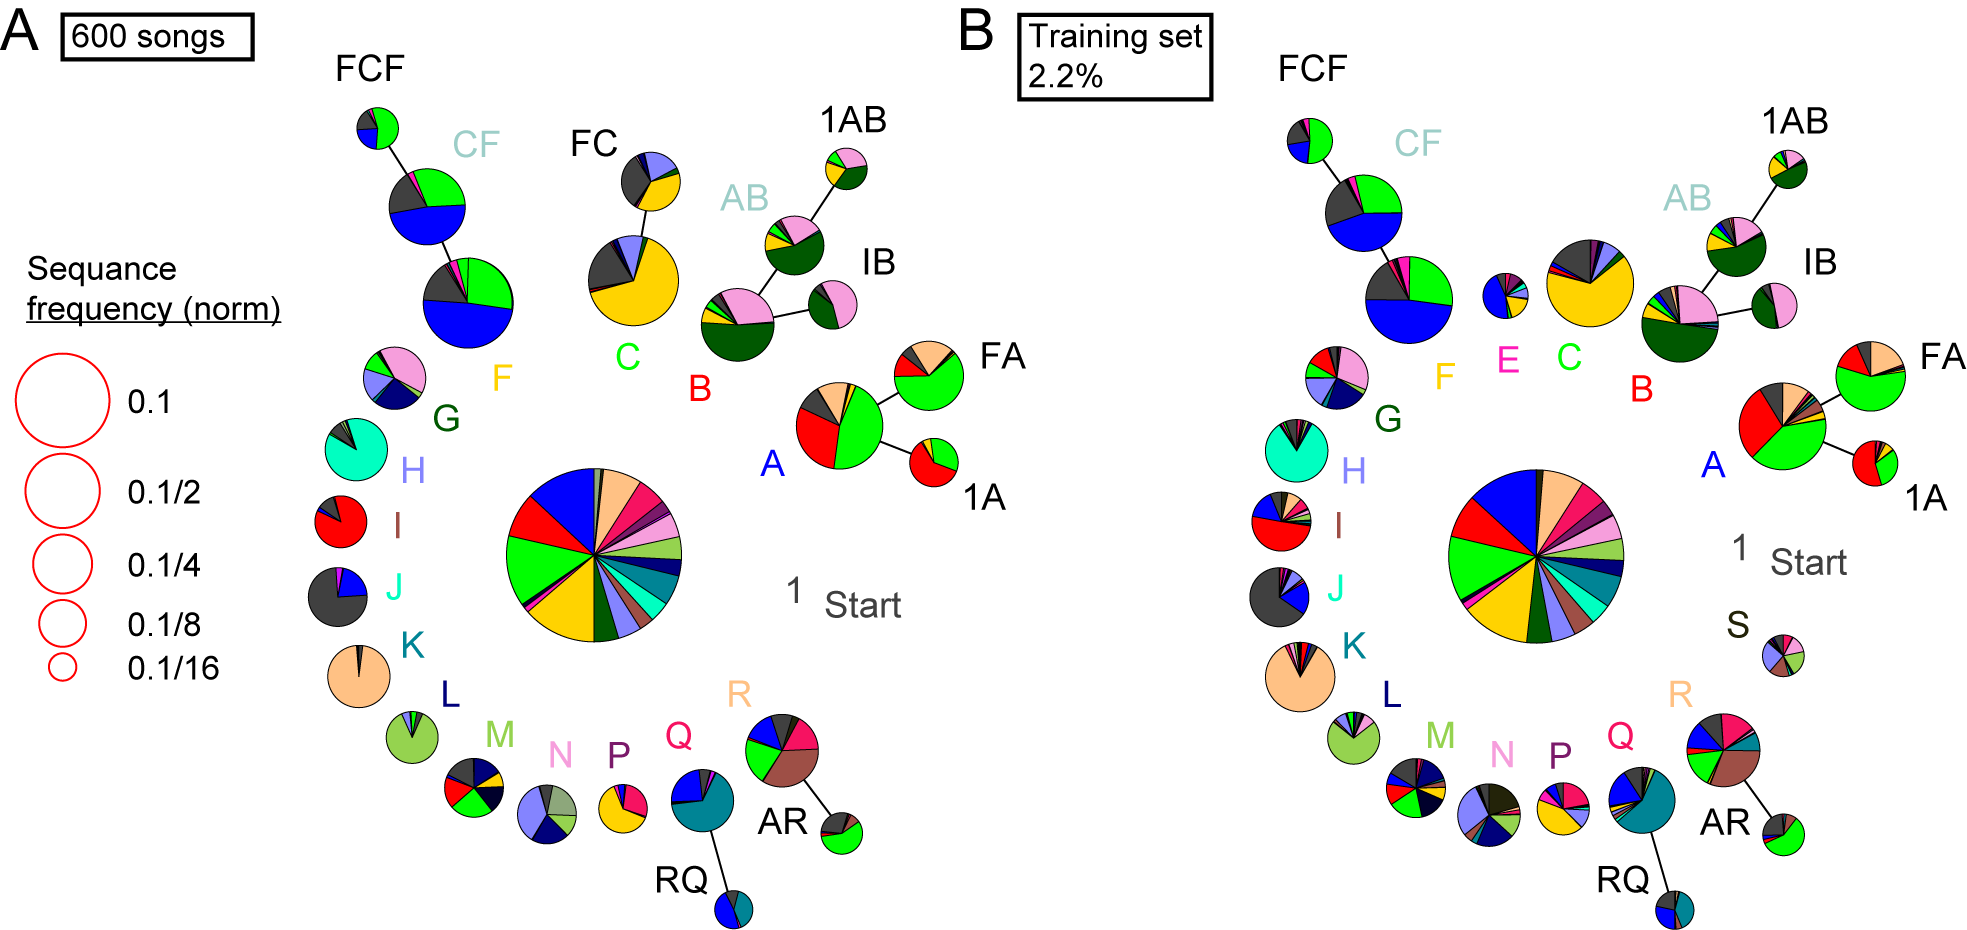
\includegraphics[scale=0.85]{Figures/fig8/Figure8_v7.png}
\caption{{\bf Example of reproducing long-range syntax dependencies, seen in \textit{Waterslager} canaries, in another strain using a TweetyNet model trained on a small fraction of the data.}
\textbf{A.} Long-range order found in 600 domestic canary songs annotated with human proof reader (methods, similar dataset size to \cite{markowitz_long-range_2013}). Letters and colors label different phrase types. Each branch terminating in a given phrase type indicates the extent to which song history impacts transition probabilities following that phrase. Each node corresponds to a phrase sequence, annotated in its title, and shows a pie chart representing the outgoing transition probabilities from that sequence. The nodes are scaled according to their frequency (legend). Nodes that can be grouped together (chunked as a sequence) without significantly reducing the power of the model are labeled with blue text.
\textbf{B.} The songs used to create the PST in A are a subset of 1764 songs. A TweetyNet model was trained using about 2.2\% of that dataset (about 9.5\% of the data in A). The PST created from the model's predicted annotation of the entire dataset is very similar to A.}
\label{fig8}
\end{figure}

\begin{figure}[!ht]
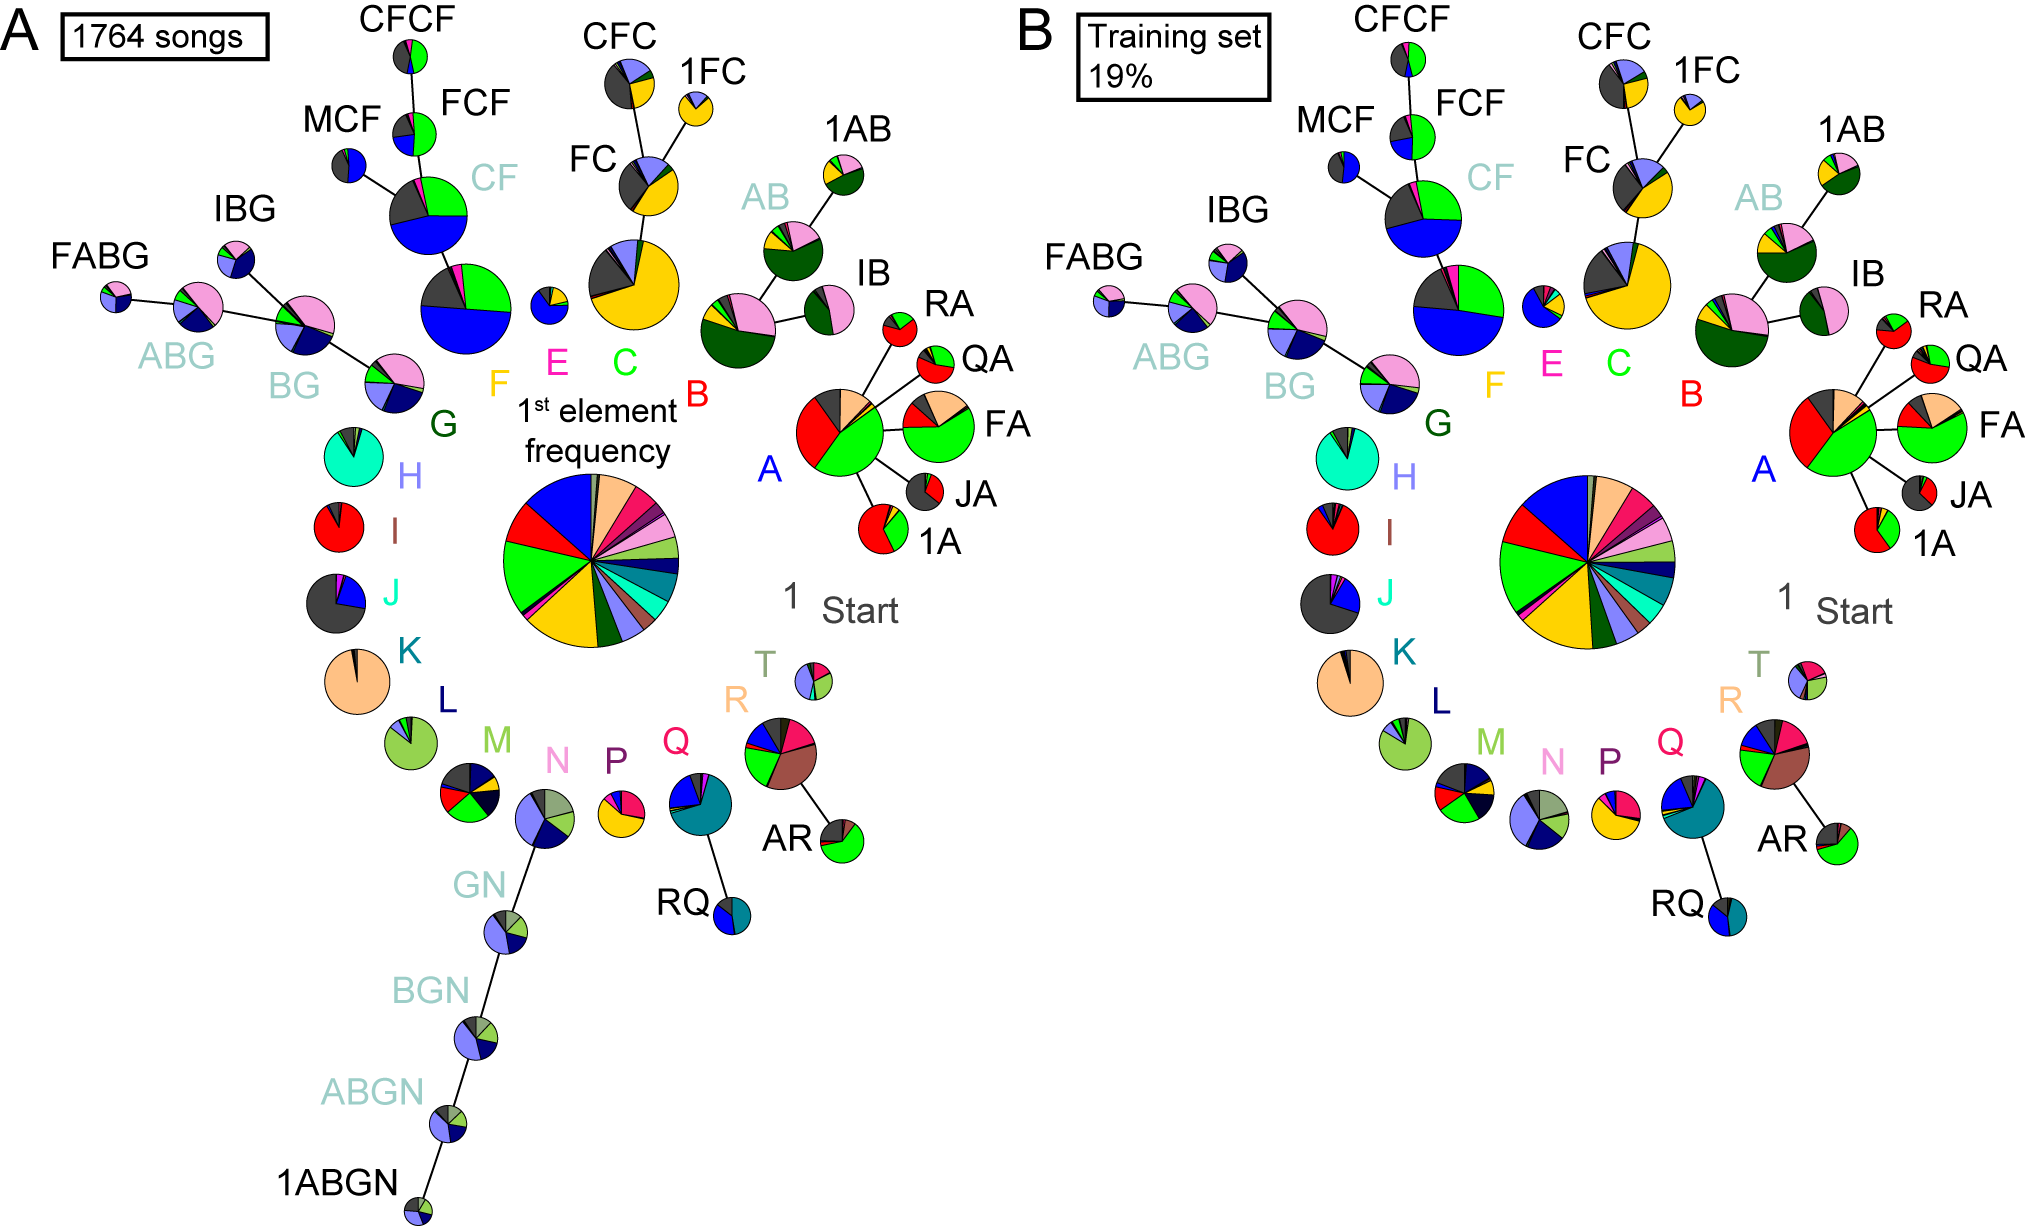
\includegraphics[scale=0.85]{Figures/fig9/Figure9_v3.png}
\caption{{\bf Example of how using TweetyNet to process a larger dataset of canary song adds detail and limits the memory of the syntax structure.}
\textbf{A.} The full dataset of 1764 songs from Fig~\ref{fig8}, annotated with a human proof reader, allowed creating a PST with greater detail. Compared to Fig~\ref{fig8}A, some branches did not grow.
\textbf{B.} An almost identical PST was created \textit{without} a human proof reader from a TweetyNet model trained on 19\% of the data. The fluctuation in transition probabilities accumulates in long sequences and, in this example, increased the minimal sequence probability included in the PST. This difference prevented the inclusion of the 'N' branch.}
\label{fig9}
\end{figure}

\begin{figure}[!ht]
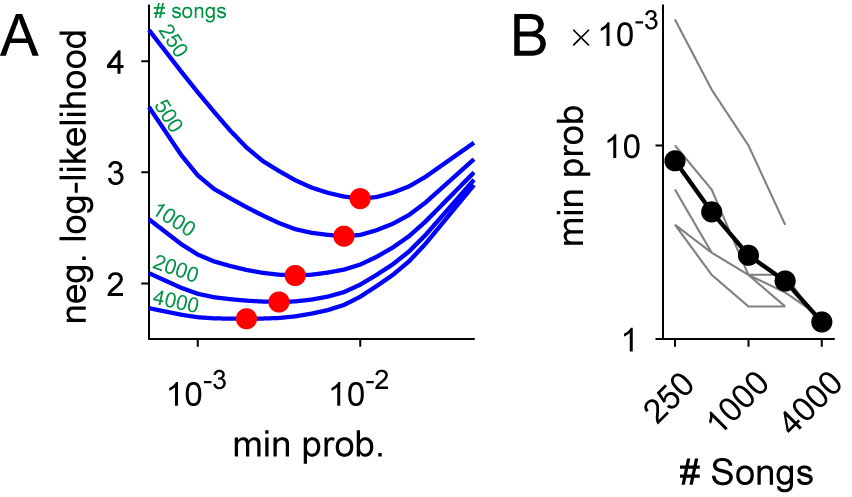
\includegraphics[scale=1.0]{Figures/fig10/Figure10_v1.png}
\caption{{\bf Using datasets more than 5 times larger than previously explored increases statistical power and the precision of syntax models.}
\textbf{A.} Ten-fold cross validation is used in selection of the minimal node probability for the PSTs (x-axis). Lines show the mean negative log-likelihood of test set data estimated by PSTs in 10 repetitions (methods). Curves are calculated for datasets that are sub sampled from about 5000 songs. Red dots show minimal values - the optimum for building the PSTs.
\textbf{B.} The decrease in optimal minimal node probability (y-axis, red dots in panel A) for increasing dataset sizes (x-axis) is plotted in gray lines for 6 birds. The average across animals is shown in black dots and line.}
\label{fig10}
\end{figure}

\subsection*{Larger data sets of annotated canary song add details and limit the memory of the syntax structure}
The increase in syntax detail, presented in Fig~\ref{fig9}, is possible because more rare nodes can be added to the PST without over-fitting the data. Formally, the PST precision increase in larger data sets is defined by the decrease in minimal node frequency allowed in the process of building PST models (Fig~\ref{fig10}), as measured in model cross validation (methods). In our data set, we find an almost linear relation between the number of songs and this measure of precision - close to a tenfold precision improvement.

In Fig~\ref{fig9}A, this increased precision allowed reliably adding longer branches to the PST to represent longer Markov chains (in comparison to Fig~\ref{fig8}A). In this example, using a dataset 3 times larger revealed a 5-deep branch that initiate with the beginning of song ('1ABGN') indicating a potential global time-in-song dependency of that transition. The PST in Fig~\ref{fig9}A also has branches that did not 'grow' when more songs were analyzed (e.g. the 'B', 'Q', and 'R' branches) - indicating a potential cutoff of memory depth that is crucial in studying the neural mechanisms of song sequence generation. 

The data sets used in Figs~\ref{fig8}A,\ref{fig9}A, and Fig~\ref{fig10}, are about 10 times larger than previous studies. To ascertain the accuracy of the syntax models, in creating the data sets we manually proof read TweetyNet's results (see methods). Across 5 different human proof readers we compare the time required to manually annotate canary song with the proof reading time and find that using TweetyNet saves 95-97.5 percent of the labor.
\newline

Taken together, the TweetyNet algorithm allowed us to annotate many more songs of individual complex singers than previously demonstrated, with high accuracy across individuals and across species. This accuracy allowed fully-automated analyses, saved most of the labor, and revealed novel details of canary syntax in a new strain.    

\section*{Discussion}
\label{Discussion}
The family of songbirds that learns by imitation consists of over 4500 species of birds. Some of these singers, such as the canary, produce songs that are much too complex to be automatically annotated with existing methods, and for these complex singers little is known about the syntax structure and organization of song. Even for birds with simple adult songs, a detailed description of song development will require the application of new methods. This is particularly true for early song development where template based extraction of song syllables and clustering of syllable forms provides an incomplete picture of the full variability of song. 

A recent study illustrated the surprises that await a more detailed analysis of song. The canary, one of the most widely bred species of domesticated songbird, was recorded for 2 hours or more and hundreds of songs were manually annotated and cross validated. This data set revealed a new complexity to the statistical structure of canary song - the song follows long-range rules where specific subsets of syllables follow transition statistics governed by 4th and 5th order Markov processes in phrase types \cite{markowitz_long-range_2013}. This rich behavior motivated another recent study to implant miniature microscopes in singing canaries, and the recorded neural signals included hierarchical memory traces corresponding to the complex syntax \cite{cohen_hidden_2020}. The sophistication of the neural representation of song in canaries was largely unanticipated based on decades of neural recordings in simpler singers.

The present project was motivated by these recent studies and the knowledge that new fundamental discoveries in vocal learning and neural dynamics will follow if automated annotation of complex song becomes possible. Some methods for automated annotation exist, but previous work suggests these methods have their own limitations, especially when applied to song with many syllable types and variable sequence such as that of Bengalese finches and canaries. 

The TweetyNet algorithm described here is a work in progress, with many clear paths for improvement. Still the first syllable error rates described here are dramatic improvements over a prior model for song parsing. We used publicly-available datasets of Bengalese finch song to benchmark TweetyNet. We showed that it achieves low error rates across many individuals. On Bengalese finch data, our single network trained end-to-end performs better than a previously proposed hybrid HMM-neural network model and does so with less training data (Fig.~\ref{fig4}). We then showed that TweetyNet models achieve low error across days, in thousands of Bengalese finch songs, even when trained with just the first three minutes of song. This experiment, while strongly restricting the data available for model training, demonstrates the usefulness of TweetyNet in 'real-life' laboratory settings - for experimentalists that want to hand annotate as little as possible. 


We next reported that TweetyNet was sufficiently accurate to reproduce the recent findings on the complex syntax structure of canary song with fully automated machine-classified song.  Specifically, a TweetyNet model trained on just 10 minutes of canary song could accurately recover the statistical structure reported from 600 manually annotated songs - exceeding 100 minutes. Furthermore, a deep network trained on 340 annotated songs, about 19\% of the data, could classify a larger data set of more than 1700 songs and build a much more complete statistical model of song revealing additional depth to the long-range syntax rules and extending prior reports on the complexity of the canary song behavior. This more complex statistical model was validated using a manually curated data set of all songs.

With a trained model performing at this level it becomes feasible to examine the effect of social context on song syntax, circadian variations in syntax, or the effects of distinct neural perturbations that could effect song syntax while keeping syllable forms intact. 
%% TBD
% Here we can discuss future directions that might improve the model, mentioning the TSNE plots, prior knowlege about song structure,e tc.
% \tododnor{This is a really important point we should make -- I moved it here from the intro because as Tim pointed out it's really a discussion point. Also we should make sure we explain that we \textbf{did} implement a simple method of post-processing, the majority vote transform, but yes clearly some method that further accounts for sequence probabilities could improve performance}
On top of sequence variations, many song studies require syllable similarity metrics to examine the effects of such neural or song pertubations, or the ontogeny of syllable forms through development. 
Here we used TweetyNet to classify the most likely syllable in every time point, focusing not on variations in syllable form but the sequential structure of song syntax. But, the syllable classification is the final processing step in TweetyNet achieved by maximum a-posteriori (MAP, or argmax) estimation following the calculation of similarity to all possible syllables. Thus, the full likelihood function that TweetyNet produces prior to classification may itself be a useful metric for syllable structure, allowing for example the time course of syllable form to be examined through development or as a result of neural perturbations. A syllable similarity metric that can be assigned at each point in time or frame of a spectrogram without syllable segmentation is, by itself, a new development in the field and can be used, in future development, to improve TweetyNet and to apply it to many more species whose song is difficult to segment. % The utility of the network outputs as a frame by frame metric of syllable similarity is illustrated in figure (canary fig). In figure (TSNE) the output vectors for Bengalese finch song segment according to syllable type. We emphasize the representation of these clusters in song do not require segmentation of song - for some species such as canaries, segmentation has been difficult to tune and even for simpler singers, the earliest subsong is contains highly variable vocalizatinos that cannot be unambiguously segmented into a discrete set of sound units.  

To make TweetyNet useful to a large research community, we developed the \texttt{vak} library - a user-friendly toolbox that enables 
researchers to apply TweetyNet simply by adapting existing configuration files. This library does not require extensive programming knowledge or expertise in neural networks. The framework will allow users to explore different methods of optimizing neural network models that might improve segmentation, and also generate alternative architectures that could incorporate distinct features and topologies. For example, in many domains transformer networks have recently replaced LSTMs for sequence processing. Substituting transformer layers for the LSTM layer could provide advances here. \cite{vaswani_attention_2017}.
Aspects of other deep networks applied to animal motor control may improve TweetyNet. Examples include object detection architectures \cite{coffey_deepsqueak_2019, mathis_deeplabcut_2018} 
applied to mouse ultrasonic vocalizations and animal motion tracking, 
and generative architectures applied to birdsong and other vocalizations 
\cite{goffinet_inferring_2019,sainburg2019animal,sainburg2019latent}. 
Lastly we note that in principle TweetyNet and \texttt{vak} library can be applied to any other annotated vocalization, including calls of bats, mouse ultrasonic vocalizations, and dolphin communication. 
We do not claim to have achieved the best possible method for automated annotation 
of vocalizations with neural networks using supervised learning methods, although 
we have aimed to establish a strong baseline for the work that will build upon ours.
That said, we are confident our method enables songbird researchers to automate annotation 
required for analyses that address central questions of sensorimotor learning.

\section*{Materials and methods}
\label{Methods}

\subsection*{Ethics declaration}
All procedures were approved by the Institutional Animal Care and Use Committees of Boston University (protocol numbers 14-028 and 14-029). Song data were collected from n = 5 adult male canaries. Canaries were individually housed for the entire duration of the experiment and kept on a light–dark cycle matching the daylight cycle in Boston (42.3601 N). The birds were not used in any other experiments.

\subsection*{Data availability}
Datasets of annotated Bengalese finch song are available at 
\url{https://figshare.com/articles/BirdsongRecognition/3470165} and  \url{https://figshare.com/articles/Bengalese_Finch_song_repository/4805749}.
Datasets of annotated canary song are available at \url{ https://datadryad.org/stash/share/lXWpizOCPjW1V63_yD8KSnj0huB-jYTJ0EfbBsNxHzU}.
Model checkpoints, logs, and source data files for figures are available at \url{https://datadryad.org/stash/share/q_N9D6dfZp_phGPQrUbeinGqcgd-lB4JZeIsd_tGXAs}

\subsection*{Code availability}
\label{methods:code}
The code implementing the TweetyNet architecture,
and code to reproduce figures in this paper, are available at
\url{https://github.com/yardencsGitHub/tweetynet}
(version 0.4.3, 10.5281/zenodo.3978389).
To aid with reproducibility of our experiments,
and to make TweetyNet more accessible to researchers studying birdsong
and other animal vocalizations, we developed a software library, 
\texttt{vak}, available at \url{https://github.com/NickleDave/vak}.
Both TweetyNet and \texttt{vak} are implemented using 
the following open-source scientific Python libraries: 
torch \cite{paszke_automatic_2017}, 
torchvision \cite{marcel_torchvision_2010}, 
numpy \cite{walt_numpy_2011, harris2020array}, 
scipy \cite{virtanen_scipy_2020}, 
dask \cite{dask_development_team_dask_2016}, 
pandas \cite{team_pandas-devpandas_2020}, 
matplotlib \cite{Hunter:2007,thomas_a_caswell_2020_4030140}, 
seaborn \cite{michael_waskom_2020_4019146}, 
jupyter \cite{kluyver2016jupyter},
attrs \cite{attrs}
and tqdm \cite{casper_da_costa_luis_2020_4054194}.

\subsection*{Data collection}
\subsubsection*{Use of available datasets}
Bengalese finch song is from two publicly-available repositories. 
The first \cite{koumura_birdsongrecognition_2016} was used for results in \ref{fig3} and can be found at 
\url{https://figshare.com/articles/BirdsongRecognition/3470165}. It accompanied the paper \cite{koumura_automatic_2016-1}.
The second \cite{nicholson_bengalese_2017} was used for results in Fig~\ref{fig4} can be found at \url{https://figshare.com/articles/Bengalese_Finch_song_repository/4805749}.
Apart from recordings made for this manuscript we used publicly available datasets of Waterslager canary songs \cite{markowitz_long-range_2013}, Bengalese finch songs \cite{koumura_automatic_2016-1} and Zebra finch songs \cite{otchy_acute_2015}.

\subsubsection*{Domestic canary song screening}
Birds were individually housed in soundproof boxes and recorded for 3-5 days (Audio-Technica AT831B Lavalier Condenser Microphone, M-Audio Octane amplifiers, HDSPe RayDAT sound card and VOS games’ Boom Recorder software on a Mac Pro desktop computer). In-house software was used to detect and save only sound segments that contained vocalizations. These recordings were used to select subjects that are copious singers ($\ge 50$ songs per day) and produce at least 10 different syllable types.
\subsubsection*{Domestic canary audio recording}
All data used in this manuscript was acquired between late April and early May 2018 – a period during which canaries perform their mating season songs. Birds were individually housed in soundproof boxes and recorded for 7-10 days (Audio-Technica AT831B Lavalier Condenser Microphone, M-Audio M-track amplifiers, and VOS games’ Boom Recorder software on a Mac Pro desktop computer). In-house software was used to detect and save only sound segments that contained vocalizations. Separate songs were defined by silence gaps exceeding 1 second.

\subsection*{Audio processing}
\subsubsection*{Segmenting annotated phrases of Waterslager canaries}
The dataset of waterslager canaries was available from a previous project in the Gardner lab \cite{markowitz_long-range_2013}. These songs were previously segmented into phrases, trilled repetitions of syllables, and not to individual syllables. To include this data in Fig~\ref{fig1} we needed to break annotated phrase segments into syllable segments. In each segmented phrase, we separated vocalization and noise fluctuations between vocalizations by fitting a 2-state hidden Markov model with Gaussian emission functions to the acoustic signal. The suspected syllable segments resulting from this procedure were proofread and manually corrected using a GUI developed in-house  (\url{https://github.com/yardencsGitHub/BirdSongBout/tree/master/helpers/GUI}).

\subsubsection*{Preparing data sets of domestic canaries}
\paragraph{Bootstrapping annotation with TweetyNet}
In this manuscript we used annotated domestic canary datasets an order of magnitude larger than previously published. To create these datasets we used TweetyNet followed by manual proofreading of its results. This process, described below, allowed 'bootstrapping' TweetyNet's performance.
\vspace{2mm}
\newline
Song syllables were segmented and annotated in a semi-automatic process:
\begin{itemize}
    \item A set of ~100 songs was manually segmented and annotated using a GUI developed in-house (\url{https://github.com/yardencsGitHub/BirdSongBout/tree/master/helpers/GUI}). This set was chosen to include all potential syllable types as well as cage noises.
    \item The manually labeled set was used to train TweetyNet (\url{https://github.com/yardencsGitHub/tweetynet}).
    \item In both the training phase of TweetyNet and the prediction phase for new annotations, data is fed to TweetyNet in segments of 1 second and TweetyNet’s output is the most likely label for each 2.7msec time bin in the recording.
    \item The trained algorithm annotated the rest of the data and its results were manually verified and corrected.
\end{itemize}
\paragraph{Assuring the identity and separation of syllable classes}
The manual steps in the pipeline described above can still miss rare syllable types of mislabel syllables into the wrong classes. To make sure that the syllable classes are well separated all the spectrograms of every instance of every syllable, as segmented in the previous section, were zero-padded to the same duration. An outlier detection algorithm (IsolationForest: \url{https://scikit-learn.org/stable/modules/generated/sklearn.ensemble.IsolationForest.html}) was used to flag and re-check potential mislabeled syllables or previously unidentified syllable classes.

\paragraph{Preparing spectrograms inputs for TweetyNet}
Spectrograms were created from audio files using custom Numpy (Bengalese finch) or Matlab (canary) code.
All spectrograms for song from a given species were created with the same parameters (e.g., number of 
samples in the window for the Fast Fourier Transform). From initial studies we found that it was necessary 
to perform standard transforms on spectrograms such as a log transform in order for the neural network to 
learn. We did not notice any difference in the nature of the transform (i.e, we also used log + 1) 
although here we do not study this systematically.

\subsection*{Network Architecture}
The network takes a 2D window from a spectrogram as input (red box, left in Fig~\ref{fig3}) and produces as output 
labels for each time bin in the window. 
The spectrogram window passes through two standard convolutional blocks, 
each of which consists of a convolutional layer and a max pooling layer. 
The convolutional layer performs a cross-correlation
like operation (asterisk in Fig~\ref{fig3}) between the spectrogram window and learned filters (greyscale boxes in Fig~\ref{fig3}) to produces feature maps.
The max pooling layer uses a similar operation to further reduce feature maps to maximum values within a sliding 
window (orange bin in Fig~\ref{fig3}). Importantly, the window size we use in the max pooling layer has a "width" of one time bin, so that this 
layer does not down-sample along the time axis (although the convolutional layer does).
The output of the second convolutional block passes through a recurrent layer made up of LSTM units, where 
the number of units equals the number of time bins in the spectrogram window.

The final layer in TweetyNet is a projection ($\overrightarrow{W}_{t,s}$) of the recurrent layer's output onto the different syllable classes, $s=1..n$, resulting in a vector of $n$ syllable-similarity scores for each spectrogram time bin $t$. The number of classes, $n$, is predetermined by the user and includes a class for no-song time bins. At present this non-song class includes both background noises and silence, and future iterations of the model may distinguish between these for better performance. To segment syllables, the bin-wise syllable-similarity scores are first used to select a single syllable class per time bin by choosing the label with the highest syllable-similarity score. Since similarity scores can be normalized, this is akin to maximum a-posteriori (MAP) label selection. Then, the labelled time bins are used to separate continuous song segments from no-song segments and to annotate each song-segment with a single label using majority decision.  

\subsection*{Training and benchmarking TweetyNet}
\label{methods:training}
Benchmarking of TweetyNet was performed with the \texttt{vak} library.
We apply standard methods for benchmarking supervised machine learning algorithms, following best practices \cite{james2013introduction}.
We leverage functionality of the \texttt{vak} library 
that extends best practices for benchmarking to the domain where 
where dataset size is measured in duration, as described in \nameref{methods:learning curves}.

\subsubsection*{Data transformations}
As stated above, the input to the network consists of spectrogram windows. To produce this input, 
we slid a window of fixed length across spectrograms, essentially creating an array of every possible 
window from each spectrogram. This array was randomly permuted then fed to the network in minibatches 
during training, along with the expected output, vectors of labels for each timebin in the 
spectrogram windows. These vectors of labeled timebins are produced programmatically by \texttt{vak} 
from annotations consisting of segment labels and their onset and offset times.
For Bengalese finch song we used windows of 88 time bins, 
and for canary song we used windows of 370 time bins.
We carried out preliminary experiments where we varied the window size 
for Bengalese finch song, but did not find that larger windows 
greatly increased accuracy, although they did increase training time.

\subsubsection*{Learning curves}
\label{methods:learning curves}
For the studies shown in Figs.~\ref{fig4},\ref{fig6}, we created learning curves,
that display a metric such as frame error rate as a function of the amount of training data.
For each individual bird we fit networks with training sets of increasing size (duration in seconds) 
and then measured performance on a separate test set.

In the case of Bengalese finches, we used training sets with durations ranging from 30-480 seconds. 
For each network trained, audio files were drawn at random from a fixed-size total training set of 900 seconds 
until the target size (e.g. 60 seconds) was reached. If the total duration of the randomly drawn audio files 
extended beyond the target duration, they were clipped at the target duration 
in a way that ensured all syllable classes were still present in the training set.
For each bird we trained ten replicates, where each 
replicate had a different subset of randomly-drawn audio files to create the target training set size.
For all Bengalese finches, we measured accuracy on a separate test set with a fixed size of 400s. We chose 
to use a totally-separate fixed-size set (instead of e.g. using the remainder of the training data set) so 
we could be sure that any variance in our measures across training replicates could be attributed to 
the randomly-drawn training set, and not to changes in the test set.
We computed metrics such as frame error rate and syllable error rate on the held-out test set for each bird.

For canaries we used test set duration of 1500-2000 seconds and training sets of 60-600 seconds for the learning curves in Fig.~\ref{fig6}. 
For the result in Table~\ref{table:1} we used a test set of 5000 seconds and a training set of 6000 seconds. 
The method for generating learning curves as just described is built into the \texttt{vak} library and 
can be reproduced using its \textit{learncurve} functionality in combination with the configuration files 
we shared (reference link) and the publicly-available datasets.

\subsubsection*{Metrics}
We measured performance with two metrics. The first is the frame error rate, that simply measures for each acoustic frame 
(in our case each time bin in a spectrogram) whether the predicted label matches the ground truth 
label. Hence the range of the frame error rate is between 0 and 1, i.e. can be stated as a percent, and 
gives an intuitive measure of a model's overall performance. Previous work on supervised sequence labeling, including 
bidirectional-LSTM architectures similar to ours, has used this metric \cite{graves_supervised_2012,graves_framewise_2005}.  

The second metric we used is commonly called the word error rate in the speech recognition literature, 
and here we call it the syllable error rate. This metric is an edit distance that counts the number of edits (insertions and deletions) needed to convert a predicted sequence into the ground-truth sequence. The error rate is normalized by dividing it by the length of the sequences.

In Table~\ref{table:1} we provide two additional measures. The first is a lower bound on the percent of all frame errors that can be attributed to slightly-misaligned syllable onsets and offsets. 
These syllable boundaries are naturally variable in creating the ground truth hand annotated data sets. Spectrogram time bins in which a trained TweetyNet model and the ground truth disagree and only one of them assigns the 'unlabeled' tag can potentially be around segment boundaries. In \nameref{S2_Fig} we show the histogram of distances, in spectrogram bins, of such frame errors from ground truth segment boundaries. The majority is concentrated in 0-2 bins away from the boundaries, amounting the overall percents summarized in Table~\ref{table:1}. The second is syllable error rate after applying post-hoc cleaning of annotation. This cleanup is done in two steps: (1) discard all segments shorter than 5msec (using 10 msec adds an insignificant improvement in some birds) and (2)assign a single label to each segment of time bins not labeled as 'silence' by majority vote.

\subsubsection*{Model output as syllable likelihoods}
In Fig~\ref{fig7} we present model outputs one step prior to assigning the most likely label to each spectrogram time bin. At that stage, one before the \textit{argmax(N)} step in Fig~\ref{fig3}, the model output for a given time bin $t$ is a real-valued affinity $a(t,s)\in\mathcal{R}$ of all predefined syllable classes $s$. In Fig~\ref{fig7} we convert these numbers to likelihoods by subtracting the minimum value and normalizing separately for each time bin $L(t,s)=\frac{a(t,s)-\min_{s'}a(t,s')}{\sum_{\sigma}[a(t,\sigma)-\min_{s'}a(t,s')]}$. This transformation was done for presentation only. Applying the commonly-used softmax transform ($x\rightarrow\frac{exp(x)}{\sum_xexp(x)}$) is equivalent since we only keep the maximal value.

\subsection*{Data analysis - song structure} 
\subsubsection*{Shared template dependence on number of syllables in song (Fig~\ref{fig1}e)}
In each bird we define an upper bound for repeating parts of songs using pairwise comparisons. For each song we examined all other songs with equal or larger number of syllables and found the largest shared string of consecutive syllables. The fraction of shared syllables is the ratio between the number of shared sequence and the number of syllables in the first, shorter, song. Then, we bin songs by syllable counts (bin size is 10 syllables) and calculate the mean and standard deviation across all pairwise comparisons.
\subsubsection*{Probabilistic suffix tree (Figs~\ref{fig8},\ref{fig9})}
For each canary phrase type we describe the dependency of the following transition on previous phrases with a probabilistic suffix tree. This method was described in a previous publication from our lab (Markowitz et. al. 2013, code in \url{https://github.com/jmarkow/pst}). Briefly, the tree is a directed graph in which each phrase type is a root node representing the first order (Markov) transition probabilities to downstream phrases, including the end of song. The pie chart in Figs~\ref{fig8},\ref{fig9} shows such probabilities. Upstream nodes represent higher order Markov chains that are added sequentially if they significantly add information about the transition.
\subsection*{Model cross validation to determine minimal node frequency}
To prevent overfitting, nodes in the probabilistic suffix trees are added only if they appear more often than a threshold frequency, $P_{min}$. To determine $P_{min}$ we replicate the procedure in \cite{markowitz_long-range_2013} and carry a 10-fold model cross validation procedure. In this procedure the dataset is randomly divided into a training set, containing 90 percent of songs, and a test set, containing 10 percent of songs. A PST is created using the training set and used to calculate the negative log likelihood of the test set. This procedure is repeated 10 times for each value of $P_{min}$, the x-axis in Fig~\ref{fig10}a. For data sets of different sizes (curves in Fig~\ref{fig10}a, x-axis in Fig~\ref{fig10}b) the mean negative log-likelihood across the 10 cross validation subsets and across 10 data sets, y-axis in Fig~\ref{fig10}a, is then used to find the optimal value of $P_{min}$ - the minimum negative log-likelihood that corresponds to the highest precision without over-fitting the training set. All PSTs in Figs~\ref{fig8},\ref{fig9} are created using the cross-validated $P_{min}$.

\section*{Acknowledgments}
This study was supported by NIH grants R01NS104925,
R24NS098536, and R01NS118424 (T.J.G.) We thank J. Markowitz and T.M. Otchy for sharing song datasets, and Nvidia Corporation for a technology grant (Y.C., Sober lab).

\section*{Supporting information}
\beginsupplement
% Include only the SI item label in the paragraph heading. Use the \nameref{label} command to cite SI items in the text.
\paragraph*{Fig. S1}
\label{S1_Fig}
{\bf Consecutive canary phrases can include acoustically-similar syllables but differ in the duration of inter-syllabic gaps.}
\begin{figure}[!ht]
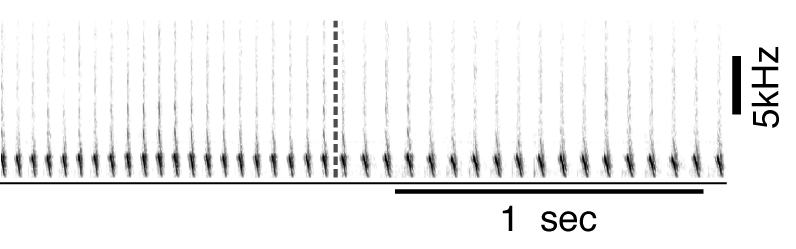
\includegraphics[scale=1.0]{Figures/Supplementaries/Supp_Figure1_1.png}
\caption{Example of two consecutive canary phrases that differ mostly in inter-syllable gaps. In this case, annotation methods that first segment syllables and then use acoustic parameters to classify them will introduce errors. By simultaneously learning acoustic and sequence properties, TweetyNet overcomes this weakness.}
\label{supp_fig_1}
\end{figure}

\paragraph*{Fig. S2}
\label{S2_Fig}
{\bf Most errors of trained TweetyNet models are disagreement on syllable boundaries of 0-2 time bins.}
\begin{figure}[!ht]
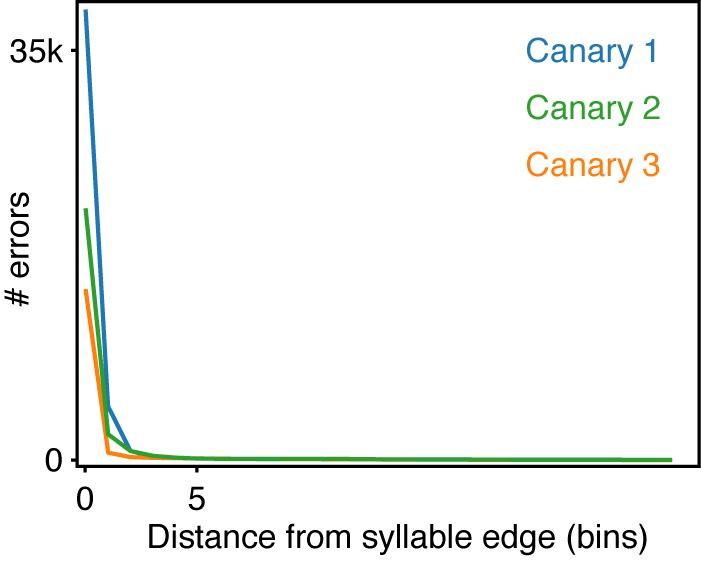
\includegraphics[scale=1.0]{Figures/Supplementaries/EdgeErrorDistCanaries.png}
\caption{Potential syllable boundary disagreements are time bins in which the ground truth test set or the trained TweetyNet model disagree and just one of them assigns the 'unlabeled' silence tag. The histograms show the distances of those time bins from the nearest syllable boundary in test sets 5000 second long.}
\label{supp_fig_2}
\end{figure}



\nolinenumbers

% Either type in your references using
% \begin{thebibliography}{}
% \bibitem{}
% Text
% \end{thebibliography}
%
% or
%
% Compile your BiBTeX database using our plos2015.bst
% style file and paste the contents of your .bbl file
% here. See http://journals.plos.org/plosone/s/latex for 
% step-by-step instructions.
% 
% \begin{thebibliography}{10}

% \bibitem{bib1}
% Conant GC, Wolfe KH.
% \newblock {{T}urning a hobby into a job: how duplicated genes find new
%   functions}.
% \newblock Nat Rev Genet. 2008 Dec;9(12):938--950.

% \bibitem{bib2}
% Ohno S.
% \newblock Evolution by gene duplication.
% \newblock London: George Alien \& Unwin Ltd. Berlin, Heidelberg and New York:
%   Springer-Verlag.; 1970.

% \bibitem{bib3}
% Magwire MM, Bayer F, Webster CL, Cao C, Jiggins FM.
% \newblock {{S}uccessive increases in the resistance of {D}rosophila to viral
%   infection through a transposon insertion followed by a {D}uplication}.
% \newblock PLoS Genet. 2011 Oct;7(10):e1002337.

% \end{thebibliography}

\bibliography{CohenNicholsonGardner2020.bib}


\end{document}

